\documentclass[pra,aps,showpacs,groupedaddress,superscriptaddress,twocolumn,toc=flat,biblatex,footinbib]{revtex4-1}
\usepackage{natbib}
\usepackage[table]{xcolor}
\usepackage[colorlinks=false]{hyperref}
\usepackage[utf8]{inputenc}
\usepackage{color}
\usepackage{bbm} 
\usepackage[english]{babel}

\usepackage{amsfonts,amsmath,amssymb,stmaryrd}

\usepackage{graphicx}
\usepackage{subfigure}  % use for side-by-side figures

%\usepackage{hyperref}
\usepackage{epsfig}
\usepackage{mathrsfs}
\usepackage{verbatim}
\usepackage{centernot}
\usepackage{ulem}
\usepackage{longtable}
\usepackage{nicefrac}
\usepackage[framemethod=tikz]{mdframed}
 
 
 %% CODE ADDED BY FABIAN:
 \bibliographystyle{apsrev4-1}
\def\bibsection{\section*{}} 

 %% CODE REMOVED BY FABIAN:
    %\usepackage{booktabs}
    %
    %\bibliographystyle{apsrev4-1}
    %\usepackage{natbib}
    % Start of 'ignore natbib' hack
    %\let\bibhang\relax
    %\let\citename\relax
    %\let\bibfont\relax
    %\let\Citeauthor\relax
    %\let\textcite\relax
    %\let\citeauthor\relax
    %\let\citeyear\relax
    %\expandafter\let\csname ver@natbib.sty\endcsname\relax
    %\usepackage[autostyle]{csquotes}
    %\usepackage[backend=biber, bibencoding=utf8, style=numeric-comp, sorting=none, maxnames=7, giveninits=true, sortcites=true, abbreviate=true, date=year]{biblatex}
    % Disable url and eprint in cases where a doi is given
    %\DeclareSourcemap{
    %  \maps[datatype=bibtex]{
    %    \map[overwrite]{
    %      \step[fieldsource=doi, final]
    %      \step[fieldset=url, null]
    %      \step[fieldset=urldate, null]
    %      \step[fieldset=eprint, null]
    %    }  
    %  }
    %}
    %% Disable ISSN
    %\DeclareSourcemap{
    %  \maps[datatype=bibtex]{
    %    \map{
    %      \step[fieldset=issn, null]
    %    }
    %    \map{
    %      \step[fieldset=title, null]
    %    }
    %    \map{
    %      \step[fieldset=month, null]
    %    }
    %  }
    %}
    
    
    %\usepackage{biblatex}
    
    %\bibliography{BibFiles/main.bib}
    %\bibliographystyle{unsrt}
    %\bibliographystyle{apsrev4-1}
    
        %\addbibresource{BibFiles/Lit.bib}

\newcommand{\note}[1]{\textcolor{blue}{(#1)}}
\renewcommand{\l}{\left(}
\renewcommand{\r}{\right)}


\newcommand{\bra}[1]{\langle#1|}
\newcommand{\ket}[1]{|#1\rangle}
\newcommand{\bkt}[2]{\left\langle #1 |#2 \right\rangle}
\renewcommand{\ij}{{\langle \vec{i}, \vec{j} \rangle}}
\newcommand{\xy}{{\langle \vec{y}, \vec{x} \rangle}}
\newcommand{\iijj}{{\langle \langle \vec{i}, \vec{j} \rangle \rangle}}
\renewcommand{\H}{\hat{\mathcal{H}}}
\newcommand{\Ht}{\tilde{\mathcal{H}}}
\renewcommand{\c}{\hat{c}}
\renewcommand{\a}{\hat{a}}
\newcommand{\s}{\hat{s}}
\newcommand{\f}{\hat{f}}
\newcommand{\cd}{\hat{c}^\dagger}
\newcommand{\rh}{\hat{\rho}}
%\newcommand{\rht}{\tilde{\rho}}
\newcommand{\ad}{\hat{a}^\dagger}
\newcommand{\sd}{\hat{s}^\dagger}
\newcommand{\fd}{\hat{f}^\dagger}
\newcommand{\bd}{\hat{b}^\dagger}
\newcommand{\ubd}{\hat{\uline{b}}^\dagger}
\newcommand{\ub}{\hat{\uline{b}}}
\renewcommand{\b}{\hat{b}}
\newcommand{\hd}{\hat{h}^\dagger}
\newcommand{\h}{\hat{h}}
\newcommand{\dd}{\hat{d}^\dagger}
\renewcommand{\d}{\hat{d}}
\newcommand{\n}{\hat{n}}
\newcommand{\D}{\hat{D}}
\newcommand{\Dd}{\hat{D}^\dagger~\hspace{-0.12cm}}

\newcommand{\G}{\hat{\Gamma}}
\newcommand{\Gd}{\hat{\Gamma}^\dagger}
\newcommand{\F}{\hat{F}}
\newcommand{\Fd}{\hat{F}^\dagger}
\newcommand{\hc}{\text{h.c.}}
\newcommand{\MF}{\text{MF}}
\newcommand{\BEC}{\text{BEC}}
\newcommand{\RG}{\text{RG}}
\newcommand{\psd}{\hat{\psi}^\dagger}
\newcommand{\ps}{\hat{\psi}}
\newcommand{\I}{\text{I}}
\newcommand{\p}{\text{p}}
\renewcommand{\sf}{\text{MIX}}
\renewcommand{\O}{\hat{\mathcal{O}}}
\newcommand{\U}{\hat{U}}
\newcommand{\W}{\hat{W}}
\newcommand{\Ud}{\hat{U}^\dagger}
\newcommand{\KP}{\text{KP}}
\newcommand{\HMF}{\mathscr{H}_{\text{MF}}}
\newcommand{\ph}{\text{ph}}
\newcommand{\IB}{\text{IB}}
\newcommand{\B}{\text{B}}
\newcommand{\eff}{\text{eff}}
\newcommand{\tr}{\text{tr}}
%MK:
\newcommand{\Zt}{$\mathbb{Z}_2$ }


\newcommand{\blankpage}{
\newpage
\thispagestyle{empty}
\mbox{}
\newpage
}

\usepackage{array}

\def\smallint{\begingroup\textstyle \int\endgroup}

\usepackage{cancel,ifthen}
\newcommand{\cmnt}[2][NoInPuT]{\ifthenelse{\equal{#1}{NoInPuT}}{}{{\color{red}\sout{#1}}} {\color{blue} #2}}
%\newcommand{\cmnt}[2][NoInPuT]{\ifthenelse{\equal{#1}{NoInPuT}}{}{{\color{red}\sout{#1}}} {\color{black} #2}}


\usepackage{bm}	% bold in math mode
\renewcommand{\vec}[1]{\bm{#1}}

%captionwidth in longtable:
\LTcapwidth=\textwidth


%%%%%%%%%%%%%%%%%%%%%%%%%%%%%%%%%%%%%%%%%%%%%%%%%%%%%%%%%%%%%%%%%%%%%%
%%%%%%%%%%%%%%%%%%%%%%%%%%%%%%%%%%%%%%%%%%%%%%%%%%%%%%%%%%%%%%%%%%%%%%
\begin{document}

\normalem	% changes \emph back to normal after introducing ulem package.

\title{Adaptive Quantum State Tomography with Active Learning}



\author{Hannah Lange}
\affiliation{Department of Physics and Arnold Sommerfeld Center for Theoretical Physics (ASC), Ludwig-Maximilians-Universit\"at M\"unchen, Theresienstr. 37, M\"unchen D-80333, Germany}
\affiliation{Munich Center for Quantum Science and Technology (MCQST), Schellingstr. 4, D-80799 M\"unchen, Germany}

\author{Matja\v{z} Kebri\v{c}}
\affiliation{Department of Physics and Arnold Sommerfeld Center for Theoretical Physics (ASC), Ludwig-Maximilians-Universit\"at M\"unchen, Theresienstr. 37, M\"unchen D-80333, Germany}
\affiliation{Munich Center for Quantum Science and Technology (MCQST), Schellingstr. 4, D-80799 M\"unchen, Germany}

\author{Maximilian Buser}
\affiliation{Department of Physics and Arnold Sommerfeld Center for Theoretical Physics (ASC), Ludwig-Maximilians-Universit\"at M\"unchen, Theresienstr. 37, M\"unchen D-80333, Germany}
\affiliation{Munich Center for Quantum Science and Technology (MCQST), Schellingstr. 4, D-80799 M\"unchen, Germany}

\author{Ulrich Schollw\"ock}
\affiliation{Department of Physics and Arnold Sommerfeld Center for Theoretical Physics (ASC), Ludwig-Maximilians-Universit\"at M\"unchen, Theresienstr. 37, M\"unchen D-80333, Germany}
\affiliation{Munich Center for Quantum Science and Technology (MCQST), Schellingstr. 4, D-80799 M\"unchen, Germany}

\author{Fabian Grusdt}
\affiliation{Department of Physics and Arnold Sommerfeld Center for Theoretical Physics (ASC), Ludwig-Maximilians-Universit\"at M\"unchen, Theresienstr. 37, M\"unchen D-80333, Germany}
\affiliation{Munich Center for Quantum Science and Technology (MCQST), Schellingstr. 4, D-80799 M\"unchen, Germany}

\author{Annabelle Bohrdt}
\affiliation{ITAMP, Harvard-Smithsonian Center for Astrophysics, Cambridge, MA 02138, USA}
\affiliation{Department of Physics, Harvard University, Cambridge, MA 02138, USA}


\pacs{}


\date{\today}

\begin{abstract}
Recently, tremendous progress has been made in the field of quantum science and technologies: different platforms for quantum simulation as well as quantum computing, ranging from superconducting qubits to neutral atoms, are starting to reach unprecedentedly large systems. In order to benchmark these systems and gain physical insights, the need for efficient tools to characterize quantum states arises. 
The exponential growth of the Hilbert space with system size renders a full reconstruction of the quantum state prohibitively demanding in terms of the number of necessary measurements. %Most physically interesting states have some internal structure, which is however challenging to exploit without a priori physical knowledge about the system and thus a potential bias.  
Here we propose and implement an efficient scheme for quantum state tomography using active learning. Based on a few initial measurements, the active learning protocol proposes the next measurement basis, designed to yield the maximum information gain. For a fixed total number of measurements and basis configurations, our algorithm maximizes the information one can obtain about the quantum state under consideration. 
We apply the active learning quantum state tomography scheme to reconstruct different multi-qubit states with varying degree of entanglement as well as to ground states of a kinetically constrained spin chain. In all cases, we obtain a significantly improved reconstruction as compared to a reconstruction based on the exact same number of measurements, but with randomly chosen basis configurations.
Our scheme is highly relevant to gain physical insights in quantum many-body systems as well as for the characterization of quantum devices, and paves the way for benchmarking and probing large quantum systems.
\end{abstract}

\maketitle

%%%%%%%%%%%%%%%%%%%%%%%%%%%%%%%%%%%%%%%%%%%%%%%%%%%%%%%%%%%%%
Since the turn of this century, the characterization of quantum states is of high importance: It is needed for assessing the performance of quantum algorithms for quantum computers, certifying the quality of experimental quantum hardware, and enables the investigation of complex quantum systems \cite{Nimbe2021, Bloch2012,Preskill2018,Altman2021}. Hence, Quantum State Tomography (QST), which is the process of reconstructing quantum states from measurements, is of high interest for both experimental and theoretical research in the field of quantum physics and quantum computing. The very nature of quantum states makes the state reconstruction a complicated task and most available techniques, e.g. linear inversion or the maximum likelihood method \cite{Haeffner2005, Hradil1997}, undergo an exponential scaling of the number of samples needed for the reconstruction with the size of the quantum system. This is due to the number of parameters containing the information about the state, which increases exponentially with system size. Therefore the application of conventional tomography methods is mostly limited to only a few qubits \cite{Abhijith2020}. 

A relatively new approach is neural network quantum state tomography. It is based on the assumption that most physical states typically have a certain degree of structure (e.g. symmetries) and can hence be described  by a reduced number of parameters. This enables the reconstruction of quantum states from less measurement data and thus tackles the main shortcoming of the aforementioned methods \cite{Carrasquilla2019,Torlai2020,Carrasquilla2021}. It has been shown that these neural network based approaches allow the reconstruction of highly entangled states with more than a hundred qubits, for example by using a restricted Boltzmann machine (RBM) \cite{Torlai2018,Melko2019}. Furthermore, machine learning based tomography is able to access observables which cannot be directly inferred from an experiment itself \cite{Torlai2019}.


Here, we show that it is possible to reduce the number of required measurement samples by using a machine learning based approach which combines restricted Boltzmann machines and active learning, see Fig.~\ref{fig:AL}. Active learning (AL) machine learning models are able to interact with their environment. In the case of QST, this interaction comprises of requesting samples which are most informative for the further learning process \cite{Settles2009}. Active learning has been applied successfully, e.g. in improving classification tasks \cite{Greiner2002, TongChang2001} or speech recognition \cite{Tur2005}, and in condensed matter theory to map out a phase diagram \cite{Ding2021}. 
Here, we use AL in the sense that our model decides actively which measurement configuration to consider for consecutive measurements in QST to improve the training most efficiently. We show that AL can highly reduce the number of samples needed for the reconstruction compared to a passive procedure relying on RBMs only. We investigate quantum states consisting of up to $19$ qubits or spin-$\frac{1}{2}$ particles which are either generated on IBM quantum devices or simulated using the density-matrix renormalization group \cite{Schollwoeck2011}. Extensions of our scheme to larger system sizes and other settings, such as fermionic systems or soft-core bosons, are straightforward.

% % % % % % % % % % % % % % % % % % % % % % % % % % % 
\begin{figure}[t]
	\centering
  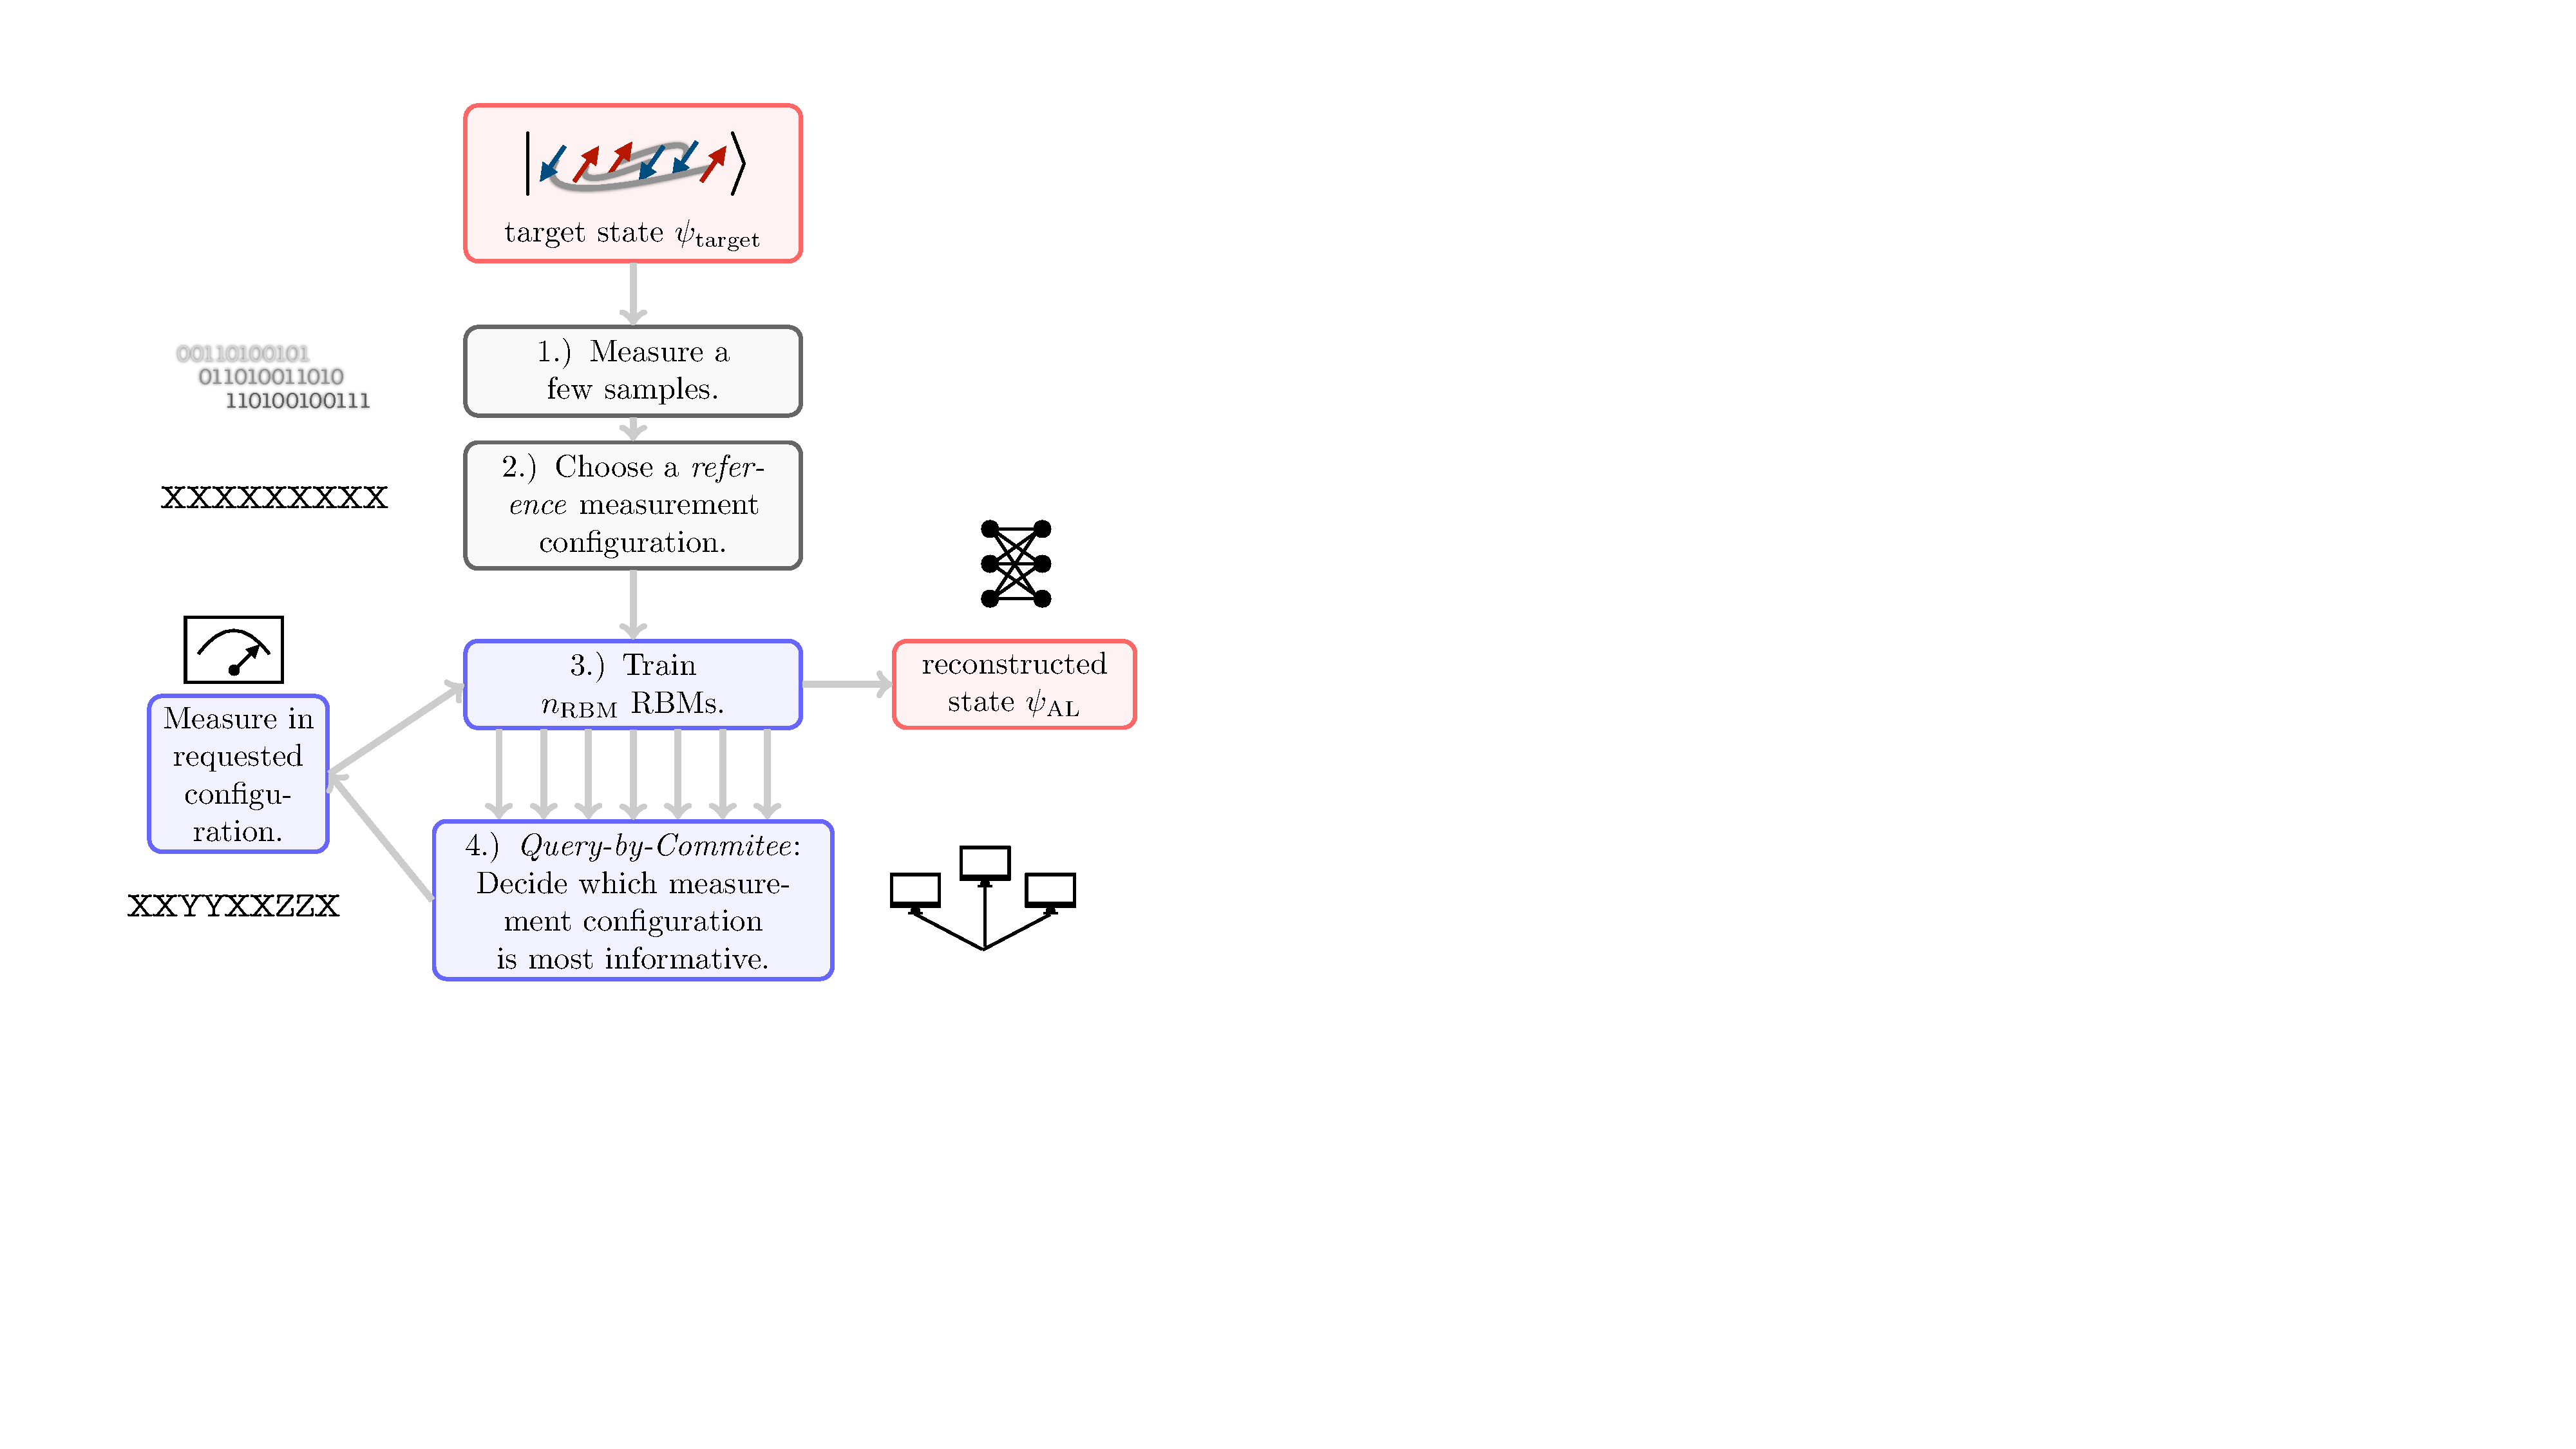
\includegraphics[width=0.495\textwidth]{Procedure2.pdf}
	\caption[Active learning procedure]{Quantum state tomography (QST) by active learning. We show our active learning cycle: In the first stage a reference measurement basis is chosen which is most suitable for reconstructing the state (grey). Then, based on the already measured data, the active learner requests specific highly informative samples (blue). These are used to train a RBM representing the reconstructed quantum state.}
	\label{fig:AL}
\end{figure}
% % % % % % % % % % % % % % % % % % % % % % % % % % % 

This article is organized as follows: we start with a brief summary of existing QST schemes by restricted Boltzmann machines, which constitute a building block of our improved active learning QST. We then introduce our active learning algorithm in section \ref{sec:Model}. In section \ref{sec:States}, we define and motivate the different quantum states considered in this work, in particular multi-qubit states with variable degrees of entanglement and ground states of a one-dimensional kinetically constrained spin chain with a hidden U(1) symmetry. We present the results of our active learning scheme for quantum state reconstruction in section \ref{sec:Results} and conclude in section \ref{sec:Summary}. 

%%%%%%%%%%%%%%%%%%%%%%%%%%%%%
\section{Restricted Boltzmann Machines}
%%%%%%%%%%%%%%%%%%%%%%%%%%%%%

Since our AL scheme also includes the training of a committee of restricted Boltzmann machines, see Fig.~\ref{fig:AL}, we will introduce them with a focus on their application to QST in this section. Here, we use the implementation of RBM quantum state tomography by Beach et al. \cite{Beach2019} in the form of a python package called QuCumber. However, the idea of our AL scheme is independent of the specific implementation of the RBMs and can in principle be applied in combination with any other quantum state tomography scheme, such as other neural network architectures \cite{Rocchetto2018,Morawetz2021,Schmale2021,Ahmed2021,Cha2021} as well as matrix-product state based state reconstruction \cite{Cramer2010,Baumgratz2013}.
Here, the target many-body quantum state is represented in terms of an artificial neural network (RBM) wave function
\begin{align}
\psi_{\mathrm{RBM}}(\vec{x})=\psi_{\lambda, \mu}(\vec{x}) = \sqrt{\frac{p_\lambda(\vec{x})}{Z_\lambda}}\mathrm{e}^{i\theta_\mu(\vec{x})/2},
\label{eq:RBMstate}
\end{align}
(see appendix \ref{appendix:RBM}), where $p_\lambda$ and $p_{\mu}=\mathrm{e}^{ \theta _{\mu}}$ are probability distributions of two RBMs with weights $\lambda$ and $\mu$ which define the amplitude and the phase of the reconstructed state. Here $\vec{x}$ labels a general set of basis states. 

A RBM consist of layers of so-called visible and hidden nodes $v_i$ and $h_j$ with bias weights $b_i$ and $c_j$. The visible nodes correspond to the input data (in our case the measurements of the target state). Both layers are connected and each connection is weighted by parameters $W_{ij}$. To reconstruct a state and represent it as a RBM, the network parameters are learned from a set of measurements. To this end, the weights $\vec{b}, \,\vec{c}$ and $\vec{W}$ are adjusted such that the probability distribution of the RBM $p_{(\lambda, \mu)}=\vert \psi_{\mathrm{RBM}}(\vec{x})\vert ^2$ become as close to the distribution of target state measurements $q(\vec{x})$ in the set of measurements $\mathcal{D}$ as possible \footnote{The empirical distribution $q(\vec{x})$ is defined as follows: if a possible outcome $\vec{v}$ is contained $N_{\vec{v}}$ times in the set of $N_{\rm tot}$ existing measurements $\mathcal{D}$, then $q(\vec{v}) = N_{\vec{v}}/N_{\rm tot}$. If $\vec{x} \notin \mathcal{D}$ has not been measured, $q(\vec{x})=0$.}. This is achieved by minimizing the so-called Kullback-Leibler divergence,
\begin{align}
KL(q, p_{(\lambda, \mu)}) = \sum_{\vec{v} \in \mathcal{D}}q(\vec{v})\mathrm{log}\frac{q(\vec{v})}{p_{(\lambda, \mu)}(\vec{v})},
\label{eq:KL}
\end{align}
which quantifies how close the reconstructed distribution $p_{(\lambda, \mu)}$ is to the measured distribution $q$.

While the Kullback-Leibler divergence can be determined without prior knowledge of the target state, benchmarking of any QST scheme requires a more direct comparison with the target state. A useful measure for the performance of the reconstruction is the fidelity
\begin{align}
    f = \vert \langle \psi_\mathrm{RBM} \vert \psi_\mathrm{target} \rangle \vert ^2,
    \label{eq:Fidelity}
\end{align}
which represents the square of the overlap of the RBM state representation and the target state \cite{QucumberDoku}. Note that the fidelity can only be evaluated if the target state vector is explicitly known. For multi-qubit systems, $f$ is often re-scaled to $\tilde{f} = f^\frac{1}{N}$, with $N$ the number of qubits, to account for the exponential size of the underlying Hilbertspace.\\

To obtain information about both the amplitude and phase of the target state, different types of measurements are required: 
\begin{itemize}
    \item[(i)] Samples from a \textit{reference} measurement configuration are needed to learn the amplitudes from the frequencies of measurements.
    \item[(ii)] Samples from measurements in further, different basis configurations are required to extract information about the phase. Each measurement in a different basis configuration corresponds to a rotation of one or several qubits into the $x$, $y$ or $z$ basis individually (see Appendix ~\ref{appendix:RBM}). 
\end{itemize} 


%%%%%%%%%%%%%%%%%%%%%%%%%%%%%
\section{Active Learning Algorithm \label{sec:Model}}
%%%%%%%%%%%%%%%%%%%%%%%%%%%%%

Depending on the properties of the quantum state under consideration, there are different configurations which contain relevant information and are hence most useful for the reconstruction. For most states it is difficult and time-consuming to obtain the optimal set of measurement configurations and amount of samples which leads to a good reconstruction (see Appendix \ref{appendix:IBM}). Here, we apply AL to choose the most informative measurement configurations during the learning process. Hereby, no a-priori information about the type of state or its properties is used. Instead, the configurations are chosen such that the amount of information contained in a finite number of measurements from this configuration is larger than for other configurations. We show that by requesting this specific, highly informative data and feeding it into the RBM, the total number of samples can be reduced while the accuracy of the machine learning model is increased compared to a procedure which uses RBMs only.   


A schematic overview of our active learning algorithm is provided in Fig.~\ref{fig:AL}. It consists of the following steps: 
\begin{itemize}
    \item[1.)] First, a few samples in three different measurement configurations are generated: without rotations ($zz\dots z$), with all qubits rotated to the $x$ axis ($xx\dots x$) and, third, with all qubits rotated to the $y$ axis ($yy\dots y$).
    \item[2.)] The reference basis for the reconstruction of the quantum state's amplitude is selected: To this end, measurements from 1.) are fed into $n_{\mathrm{RBM}}$ RBMs. In general, the reference basis is chosen to be the basis where the $n_{\mathrm{RBM}}$ RBMs agree most on the wave function's state vectors. More precisely, the configuration with the lowest variance of the RBM state vector's entries is chosen. Depending on the size of the Hilbert space, this can be achieved by directly comparing the state vectors, or by sampling from the $n_{\mathrm{RBM}}$ RBMs and comparing the resulting distributions. 
    %For states where the state vector is known (see Eqs.~\eqref{eq:State1} to \eqref{eq:State3}), the configuration with the highest overlap (fidelity) between the $n_{\mathrm{RBM}}$ RBM wave function's state vectors and target state vector is chosen to be the reference basis.
    \item[3.)] Third, we
    train $n_{\mathrm{RBM}}$ different RBMs on the data in the pool of samples using the open source python package QuCumber \cite{Beach2019}.
    \item[4.)] The active learner requests measurements in a configuration which improve the reconstruction most efficiently. Here we apply the so called \textit{query-by-commitee} strategy and request samples from those configurations for which the RBMs disagree most: This is decided based on the variances of the amplitudes and phases between different RBMs. \begin{itemize}
        \item [a)] If the RBMs disagree more on the amplitudes than on the phases of the reconstructed states (i.e. the variance of the amplitudes is larger than the variance of the phases of $\psi_{\mathrm{RBM}}$ for different RBMs), the active learner requests measurements from the reference basis.
        \item [b)] Else, the probability distributions $p_{(\lambda_i, \mu_i)}(\vec{x})=\vert \psi_{\mathrm{RBM}i}(\vec{x})\vert ^2$ with $\psi_{\mathrm{RBM}i}$ rotated to $n$ different configurations for all $i = 1, \dots, n_{\mathrm{RBM}}$ RBMs (each RBM characterized by its set of parameters $\lambda_i, \, \mu_i $) is used to select the next measurement basis. Here, we calculate the RBM probability distributions in up to $n\leq 2^N$ ($N$: system size or number of qubits) different configurations. Then, the active learner evaluates for which measurement configuration the RBMs disagree most on the probability distributions $p_{(\lambda_i, \mu_i)}$. To this end, for each measurement configuration the variance of the probabilities for each measurement outcome between the different RBMs is evaluated and summed up. The configuration with the highest variance is considered to be the most controversial between all RBMs and is selected as the next measurement configuration.
    \end{itemize} 
    \item[5.)] Measure samples in the requested configuration and repeat steps 3.) and 4.) until the accuracy of the model reaches a predefined standard, or the predefined maximum number of measurements is reached.
\end{itemize}


%%%%%%%%%%%%%%%%%%%%%%%%%%%%%
\section{Considered States \label{sec:States}}
%%%%%%%%%%%%%%%%%%%%%%%%%%%%%
Before we present results by our AL-QST scheme, we provide an overview of the quantum states used to benchmark our method. We chose two types of states: first a set of generic qubit states with variable degree of entanglement, which provide direct insights into the performance of our scheme. Second, we consider many-body ground states of a one-dimensional spin Hamiltonian as an illustration of our method for quantum simulators. 

%%%%%%%%%%%%%%%%%%%%%%%%%%%%%%
\subsection{Qubit states and IBM's Quantum cloud}

We investigate the reconstruction of states which are generated on real quantum devices and classical simulators of the \textit{IBM Quantum} platform \cite{IBM}. IBM provides 21 quantum systems based on superconducting qubits which can be accessed via a cloud. Systems with up to five qubits are accessible for non-internal users with a free account. Using Qiskit it is possible to implement quantum algorithms on these quantum systems \cite{Qiskit2010}.

Here, we consider the reconstruction of three target states:
\begin{itemize}
\item \textit{Greenberger–Horne–Zeilinger} (GHZ) states, 
    \begin{align}
    \ket{\mathrm{GHZ}} = \frac{1}{\sqrt{2}} \left(\ket{0\dots 0} + \ket{1\dots 1} \right),
    \label{eq:State1}
    \end{align} 
\item polarized product states with all qubits set to one (\textit{spins up}),
\begin{align}
    \ket{\mathrm{spins}\,\mathrm{up}} = \ket{1\dots 1},
    \label{eq:State2}
\end{align}
\item and states with a state vector with equal amplitudes for all components (\textit{equal probability}), e.g. for two qubits
\begin{align}
    \ket{\mathrm{equal}\,\mathrm{prob}} = \frac{1}{2} \ket{00}+  \frac{1}{2} \ket{01} +  \frac{1}{2}   \ket{10} +  \frac{1}{2}  \ket{11}.
    \label{eq:State3}
\end{align}
\end{itemize}

Using the IBM platform we investigate the reconstruction of states with five qubits. Tools for rotating and measuring the quantum systems are provided by Qiskit. An example for measuring a two-qubit system in the $xy$ basis (first qubit rotated to the $x$ axis, second qubit rotated to $y$) is shown in Appendix \ref{appendix:RBM}. In the following sections we will use the same notation, where e.g. $xx\dots x$ denotes a system with all qubits rotated from the $z$ to the $x$ axis.

We also consider the above states with $N>5$ qubits. In this case, we represent the wavefunctions by matrix product states using the SyTen package \cite{syten1,syten2}.

%%%%%%%%%%%%%%%%%%%%%%%%%%%%%
\subsection{Kinetically constrained spin chain}
As an illustrative example, we apply AL-QST to reconstruct ground states of a kinetically constrained one-dimensional spin chain (KCS) model. It is described by the following Hamiltonian \cite{Iadecola2020,Borla2020,Kebric2021}:
\begin{align}
    \H = t \sum_{j=2}^{L-1} &\l 4 \hat{S}^{x}_{j-1} \hat{S}^{x}_{j+1} - 1 \r \hat{S}^{z}_j \nonumber \\
    &- h \sum_{j=1}^{L} 2 \hat{S}^{x}_{j}
    + \mu \sum_{j=2}^{L} \hat{S}^{x}_{j-1} \hat{S}^{x}_{j},
    \label{eq:LGT_Model_Spin_Def}
\end{align}
where $\hat{S}^\mu_j$ denotes a spin-$1/2$ operator ($\mu=x,y,z$) on site $j=1,...,L$. This model has a very interesting interpretation, where the spin domain walls in the $x$-basis correspond to particles on a dual lattice.
More precisely, model \eqref{eq:LGT_Model_Spin_Def} can be mapped to a one-dimensional \Zt lattice gauge theory with matter \cite{Borla2020}, see Appendix \ref{ApdxKinConsSpn}.

We choose the system in Eq.~\eqref{eq:LGT_Model_Spin_Def} due to several non-trivial properties for which we can check in the reconstructed state. These include: (i) that the underlying excitations are domain walls of the spins, extending beyond one site -- a fact that needs to be captured by a reliable QST scheme; (ii) the Hamiltonian features a hidden U(1) symmetry describing the conservation of the total number of domain walls -- their number is controlled by the chemical potential $\mu$; (iii) the model hosts gapless Luttinger liquids with significant amount of non-local entanglement, presenting a general challenge for any QST scheme; and (iv) by tuning the effective field from $h=0$ to $h \neq 0$, a confinement-deconfinement transition exists where the nature of constituents of the Luttinger liquid changes, as indicated by a change of the Fermi momentum $k_{\rm F}$ and reflected in the period of Friedel oscillations \cite{Borla2020,Kebric2021}.

Below we compute the ground states of Eq.~\eqref{eq:LGT_Model_Spin_Def} with the density-matrix renormalization group (DMRG) using the SyTen package \cite{syten1,syten2}. We obtain a matrix-product state (MPS) representation of the ground states, from which efficient snapshot sampling is possible \cite{Ferris2012}, including in variable bases \cite{buser2021arXiv}. This provides us with the data required to run and benchmark the AL-QST algorithm.

To probe how close the reconstructed state is to the actual ground state, we compute the following observables. We start with the local domain-wall density,
\begin{equation}
    \hat{n}(j) = \frac{1}{2}
    \l 1 - 4 \hat{S}^{x}_{j}\hat{S}^{x}_{j+1} \r.
    \label{eq:LocalDensitySpinDef}
\end{equation}
This also immediately leads us to the conserved total system density $\hat{n}^{\rm tot} = \frac{1}{L-1} \sum_{j=1}^{L-1} \hat{n}(j)$. In practice, we find it convenient to define a vector $\vec{n}$ of local densities with the following entries,
\begin{equation}
    \vec{n} = \bigl( \langle \hat{n}_{1} \rangle, \langle \hat{n}_{2} \rangle, ..., \langle \hat{n}_{L} \rangle \bigr)^T.
\end{equation}

In order to probe the confinement of domain walls we consider their non-local equal-time Green's function measured relative to the center $L/2$ (for $L$ odd: $L/2+1/2$) of the chain (see Appendix \ref{ApdxKinConsSpn} for more details):
\begin{multline}
    c(d) = \left \langle
    \frac{1}{2} \l 1 - 4\hat{S}^{x}_{L/2}\hat{S}^{x}_{L/2+1} \r \l \prod_{L/2 < j \leq L/2+d}
    2 \hat{S}^{z}_{j} \r  \right. \\
   \times \left. \frac{1}{2} \l 1- 4\hat{S}^{x}_{L/2+d}\hat{S}^{x}_{L/2+1+d} \r
    \right \rangle .
    \label{eq:GreensSpinDef}
\end{multline}
We highlight the following key properties of this function: (a) for distance $d=0$, the density is recovered, $c(0) = \langle \hat{n}(L/2) \rangle$; (b) the decay of $c(d)$ allows to distinguish between confined (exponential decay) and deconfined (power-law decay) regimes.




% % % % % % % % % % % % % % % % % % % % % % % % % % % 
\begin{figure}[t]
	\centering
  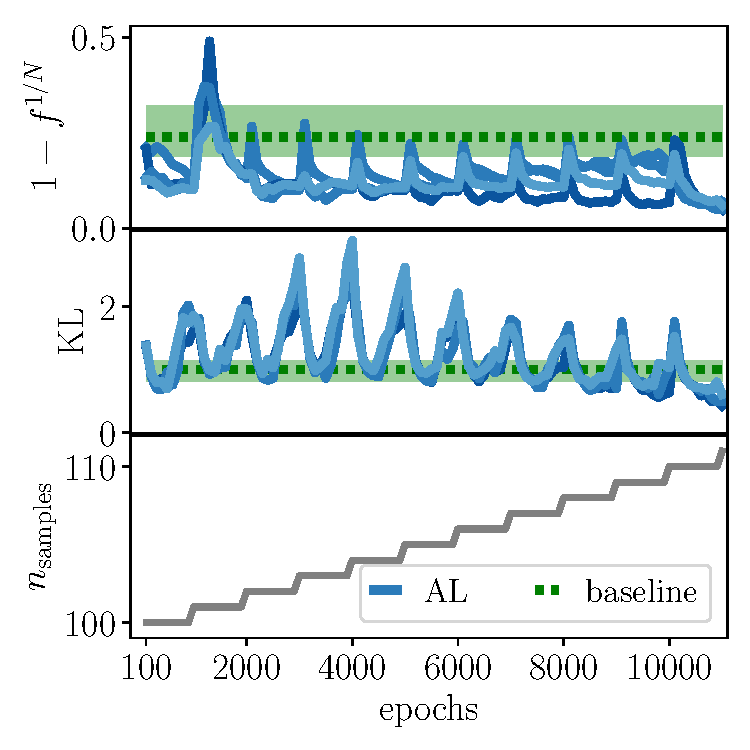
\includegraphics[width=0.48\textwidth]{Paper/Graphics/LearningCurve.pdf}
	\caption[Learning curve with active learning]{Learning curve: re-scaled fidelities (top), Kullback-Leibler divergence (middle) and number of samples within the learning cycles (bottom) with active learning for a GHZ state with $9$ qubits. Here, $4$ different RBMs are used in step 4.) of the active learning cycle (blue lines). At the end, $110$ samples were used. The results can be compared to a learning cycle without active learning (green). The green band corresponds to the entire span of results without AL. The active learner decided to choose the $zz\dots z$ basis as reference basis in step 2.) and requested measurements from $10$ additional configurations (step 4.)).}
	\label{fig:ALLearningCurve}
\end{figure}
% % % % % % % % % % % % % % % % % % % % % % % % % % % 


%%%%%%%%%%%%%%%%%%%%%%%%%%%%%
\section{Results\label{sec:Results}}
%%%%%%%%%%%%%%%%%%%%%%%%%%%%%
The active learning curve for an exemplary state (GHZ state with $9$ qubits) is shown in Fig.~\ref{fig:ALLearningCurve}. The results for AL tomography are compared to QST without active learning (denoted \textit{baseline}) by using the pure RBM reconstruction of QuCumber, the same number of samples as for AL and equally many, but randomly chosen measurement configurations. Note that we consider the number of samples and configurations at the end of the AL scheme for the baseline reconstruction. Hence, the results for AL and baseline can differ already at the beginning of the training. The pool of samples which is used for the RBM training is the same for all RBMs (both for AL and baseline, respectively).\\

Fig.~\ref{fig:ALLearningCurve} shows the learning curve for the AL scheme as presented in Fig.~\ref{fig:AL}. After the selection of the reference configuration ($zzzzzzzzz$, not shown in Fig.~\ref{fig:ALLearningCurve}) the training starts with $100$ samples drawn from the reference basis, which are fed into the QuCumber state reconstruction as implemented by Beach et al. \cite{Beach2019} (see step 3.). In the subsequent learning sequence the re-scaled fidelity $f^{1/N}$ increases ($1-f^{1/N}$ decreases) and the Kullback-Leibler divergence $KL$ decreases. However, the samples measured in step 1.) of the active learning routine do not contain enough information to decrease $1-f^{1/N}$ below a threshold value of $10\, \%$ (see first section in Fig.~\ref{fig:ALLearningCurve}). Moreover, the lack of information in the training set can be seen from the fact that both quantities increase at the end of the first section instead of decreasing. 

After that, more and more samples are added to the pool of measurements which are requested by the learner and the RBM learning process is re-started (with the same initialisation of the RBMs as before). For example, the learner requests a measurement from the $xxyzzyxzz$ configuration after the first learning cycle, and $xyzzyzxzx$ after the second cycle. Step by step, the learning curve drops and increases again with every query. This process is stopped when a specified re-scaled fidelity (here $f^{1/N}_{\mathrm{stop}}=90\, \%$) is reached or the number of posed queries exceeds $30$. The final fidelity in this example is $f^{1/N}=94.29 \pm 0.09
\,\%$ (average over the four RBMs used for step 3.)) using only $110$ samples and three configurations. 

A learning procedure without AL with the same number of measurements and equally many, but randomly chosen configurations ends with $f^{1/N}_{\mathrm{baseline}}=76.11\pm 5\,\%$ (average over four RBMs, all of them trained with the same samples), indicated by the dotted line in Fig.~\ref{fig:ALLearningCurve}. Hence, the quality of the reconstruction was improved strongly by the use of active learning. Furthermore, the span of outcomes for different RBMs is significantly decreased compared to a learning procedure without active learning (visualised by the green band in Fig.~\ref{fig:ALLearningCurve}), which makes the results much more reliable than without AL. 

Depending on the state under investigation and its properties, the learning curve can differ from the one in this example, e.g. with regimes where the difference between reconstructed and target state stagnates or even grows. This is not unintentional within our learning scheme: If a new sample is requested that contains completely different information (i.e. if one sample measured in $xx\dots x$ is added to a pool of samples from $zz\dots z$) the learner may get confused in the first place. However, when requesting more and more samples afterwards, the same piece of information can become a valuable contribution to a good reconstruction (see Fig.~\ref{fig:Example_GHZIBMclassical}).  Other exemplary curves can be found in the Appendix.\\


In the following sections, the results for the active learning procedure as explained in section \ref{sec:Model} will be presented for states on IBM's quantum devices and states generated with DMRG. The number of samples $N_{\mathrm{tot}}$, number of queries $N_{\mathrm{queries}}$, number of samples per query $N_{\mathrm{per\,query}}$ and number of different configurations $N_{\mathrm{config}}$ are presented in Tab.~\ref{tab:Samples_IBM} and \ref{tab:Samples_DMRG}. Based on our experience that for a good reconstruction of the amplitude in most cases more information about the reference configuration is needed (compared to the reconstruction of the phase based on locally rotated configurations), we request more samples than $N_{\mathrm{per\,query}}$ (if not stated differently $3\cdot N_{\mathrm{per\,query}}$) if the reference configuration is requested.


\subsection{Tomography results for quantum states on IBM's Quantum cloud \label{sec:States_IBM}}

% % % % % % % % % % % % % % % % % % % % % % % % % % % 
\begin{figure}[t]
	\centering
  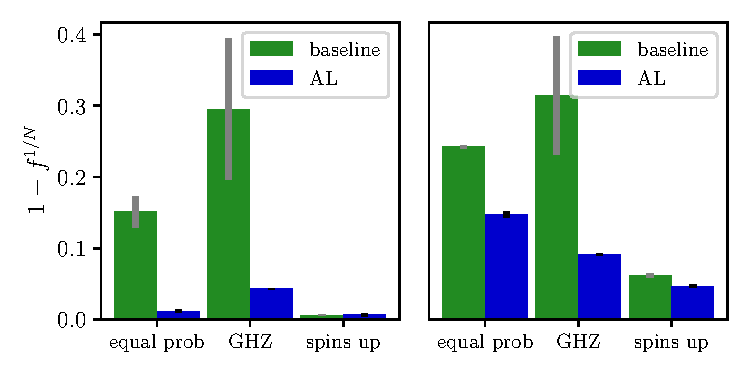
\includegraphics[width=0.48\textwidth]{Paper/Graphics/rescaled_fidelity.pdf}
	\caption[]{Final re-scaled fidelities the states defined in Eqs.~\eqref{eq:State1}, \eqref{eq:State2} and \eqref{eq:State3} with $5$ qubits generated on classical quantum simulators (left) and real quantum devices (right). An exemplary learning curve can be found in Fig.~\ref{fig:Example_GHZIBMclassical}.}
	\label{fig:IBM}
\end{figure}
% % % % % % % % % % % % % % % % % % % % % % % % % % % 

% % % % % % % % % % % % % % % % % % % % % % % % % % % 
\begin{figure}[t]
	\centering
  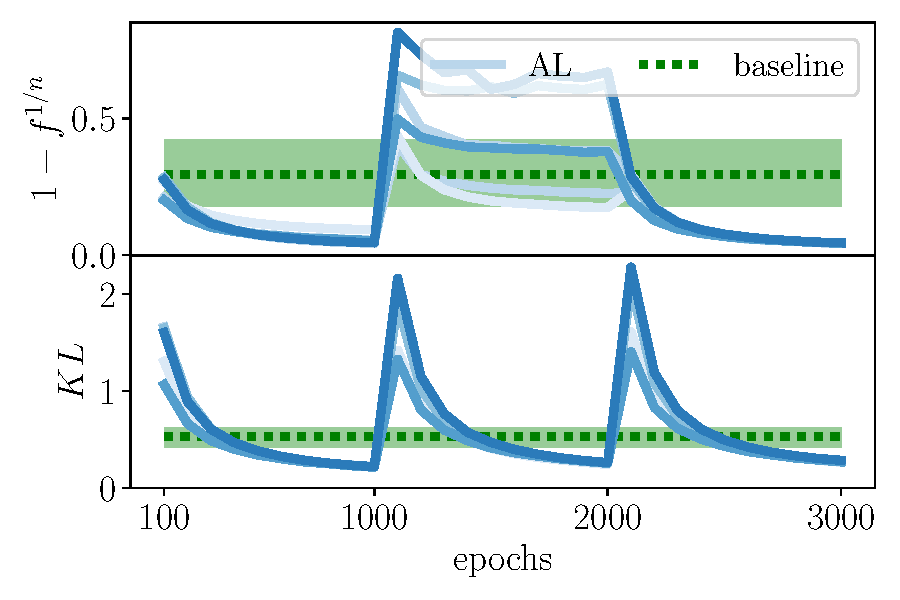
\includegraphics[width=0.48\textwidth]{Paper/Graphics/classical_GHZ.pdf}
	\caption[]{Examplary learning curves for the GHZ state (see Eq.~\eqref{eq:State2}) with $5$ qubits generated on a classical quantum simulator by IBM.}
	\label{fig:Example_GHZIBMclassical}
\end{figure}
% % % % % % % % % % % % % % % % % % % % % % % % % % % 

In this section the results for states defined in \eqref{eq:State1}, \eqref{eq:State2} and \eqref{eq:State3} generated on IBM's classical quantum simulator, which is designed to  mimic the execution of an actual device, and on real quantum devices are presented (for more details see appendix~\ref{appendix:IBM}). We consider a system size of $5$ qubits. The reconstruction results can be found in Fig.~\ref{fig:IBM}. Here the training is stopped as soon as $f^{1/N}_{\mathrm{stop}}=90\,\%$ is reached for the classical quantum simulators. For the real devices, $f^{1/N}_{\mathrm{stop}}=80\,\%$ is used (except for the GHZ state with $f^{1/N}_{\mathrm{stop}}=90\,\%$). The number of samples, queries and configurations at the end of the training is presented in Tab.~\ref{tab:Samples_IBM}.

%For the equal probability state the fidelity is improved by around $15\,\%$ to $96.01\pm 0.37\,\%$ when generated on a classical quantum simulator (by $5\,\%$ to $93.79\pm 0.47\,\%$ for the quantum device). Here reference basis was selected to be $xxxxx$ ($zzzzz$ for quantum devices). 

When reconstructing the GHZ state with AL, the active learner selects the $zzzzz$ basis as the reference basis. The fidelity of the GHZ classical quantum simulator states is improved by around $25\,\%$ from $f^{1/N}=1\pm20\,\%$ without AL to $f^{1/N}=96.10\pm0.16\,\%$. For real quantum devices the quality of the reconstruction improves as well, by around $22\,\%$ from $f^{1/N}=68.6\pm8.3\,\%$ without AL to $f^{1/N}=90.93\pm0.16\,\%$. Moreover, the standard deviation of the results for different RBMs is lowered by up to two order of magnitude for the classical quantum simulators and quantum devices, which makes the results more robust when using AL.

For the state with all spins pointing upwards (all qubits having value one), the reference basis containing the most valuable information about the state is the $zzzzz$ basis. When using AL, this configuration is selected and the results are extremely good already in the first cycle of AL, with a fidelity of $f^{1/N}=99\,\%$ for simulator and real device. The QuCumber reconstruction without AL coincidentally uses the $zzzzz$ reference basis by default and hence coincidentally the perfect reference basis for the reconstruction of this state. Therefore, no difference between AL compared to the baseline can be observed.

For the state with equal probabilities, the reconstruction results are improved as well. Here, the $xxxxx$ basis is chosen and the fidelity is increased by $14\,\%$ to $f^{1/N}=98.841\pm 0.022\,\%$ for simulated states ($10\,\%$ to $f^{1/N}=85.28\pm 0.40\,\%$ for real quantum devices). Furthermore, the variance is decreased by a factor of up to $10$. In contrast to the GHZ state, where the improvement is achieved by increasing the fidelity step by step with every query, for this system the underlying reason for the improvement is the rotation of the reference configuration: When the equal probability state is rotated from the $zz\dots z$ configuration to the $xx\dots x$ configuration, the measurement distribution changes from equally distributed peaks for all outcomes to a peaked distribution at $00\dots 0$. Similarly to the state with all spins up, it is relatively easy for the RBMs to learn this distribution. 


In Fig.~\ref{fig:Example_GHZIBMclassical} the learning curve for the GHZ state is shown. When using AL the fidelity and $KL$ divergence are decreased strongly at the end of the training. One can see that in the first learning cycle, which uses $60$ samples drawn from the $zzzzz$ reference basis, the information contained in these samples is not enough to decrease the fidelity below the threshold value of $f^{1/N}_{\mathrm{stop}}=90\,\%$ for most RBMs. By adding only one sample of the $yzzzy$ configuration to the pool of samples in the first query, the RBMs can not make sense of the phase information that is added and the fidelity increases compared to the first learning step. However, one can see that the RBMs still adapt to the new information since the $KL$ is decreased to a comparable amount as in the first part of the learning. In the second query one sample from $xxyxy$ is added. Together with the other samples, the information contained in the measurements is enough to adapt the phase of the reconstructed wave function such that  the fidelity increases above the threshold value. 

% % % % % % % % % % % % % % % % % % % % % % % % % % % 
\begin{table}[]
\begin{tabular}{l|ccc|ccc}
           & \multicolumn{3}{c|}{classical quantum sim.} & \multicolumn{3}{c}{quantum device} \\
           & $N_{\mathrm{tot}}$ & $N_{\mathrm{queries}}$         & $N_{\mathrm{config}}$      & $N_{\mathrm{tot}}$     & $N_{\mathrm{queries}}$   & $N_{\mathrm{config}}$       \\\hline
GHZ        &    $62$            &    $2$               &     $3$    &    $102$          &   $2$  &     $3$                 \\
equal prob &    $2$            &   $1$                   &     $0$ &     $2$         &   $1$           &     $0$        \\
spins up   &   $4$             &     $1$ &     $0$                &        $4$      &    $1$   &     $0$              
\end{tabular}
\caption{Number of samples $N_{\mathrm{tot}}$, number of queries $N_{\mathrm{queries}}$ and configurations $N_{\mathrm{config}}$ selected by the active learner for the reconstruction of the quantum states generated on IBM's classical quantum simulators and quantum devices. Here, the number of samples is $N_{\mathrm{per\,query}}=1$ and the reference configuration selected by the AL is $zz\dots z$ for spins up and GHZ states, and $xx\dots x$ for the equal probability state. GHZ, equal probability and spins up states are defined in Eqs.~\eqref{eq:State1} to \eqref{eq:State3}.}
\label{tab:Samples_IBM}
\end{table}
% % % % % % % % % % % % % % % % % % % % % % % % % % % 


\subsection{Tomography results for DMRG states}
% % % % % % % % % % % % % % % % % % % % % % % % % % % 
\begin{figure}[t]
	\centering
\begin{minipage}[t]{0.23\textwidth}
   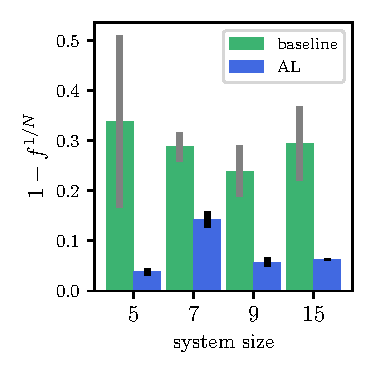
\includegraphics[width=1\textwidth]{Paper/Graphics/GHZ_rescaled_fidelity.pdf}
\end{minipage}
\begin{minipage}[t]{0.23\textwidth}
   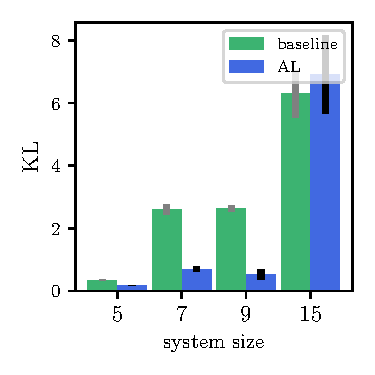
\includegraphics[width=1\textwidth]{Paper/Graphics/GHZ_KL.pdf}
\end{minipage}
\caption[]{Re-scaled fidelity (left) and KL (right) for GHZ states with $5$ to $15$ qubits generated with SyTen \cite{syten1,syten2}. An exemplary learning curve for $9$ qubits is shown in Figs.~\ref{fig:ALLearningCurve} and for $15$ qubits in \ref{fig:Example_GHZ15_MPS}.}
 \label{fig:GHZ_pyten}
\end{figure}

\begin{figure}[t]
	\centering
  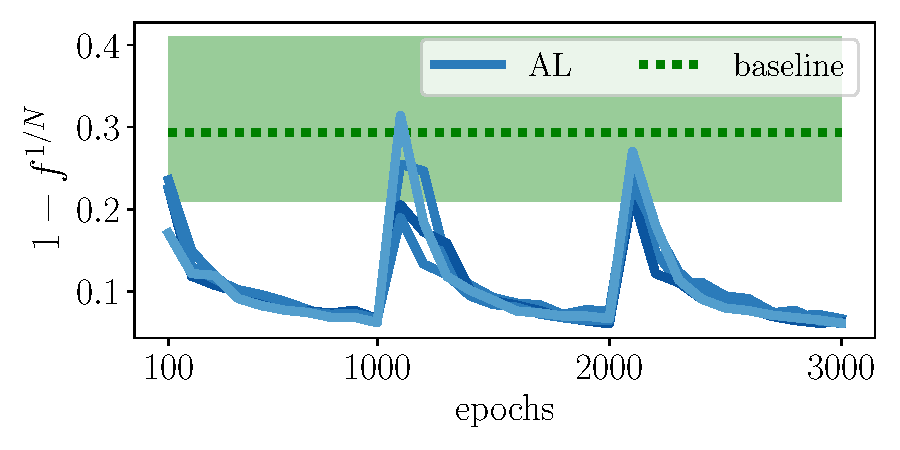
\includegraphics[width=0.48\textwidth]{Paper/Graphics/GHZ_fidelity_15_qubits_summary.pdf}
	\caption[]{Examplary learning curves for the GHZ state (see eq. \eqref{eq:State3}) with $15$ qubits generated with SyTen.}
	\label{fig:Example_GHZ15_MPS}
\end{figure}

% % % % % % % % % % % % % % % % % % % % % % % % % % % 


% % % % % % % % % % % % % % % % % % % % % % % % % % % 
\begin{figure}[t]
	\centering
   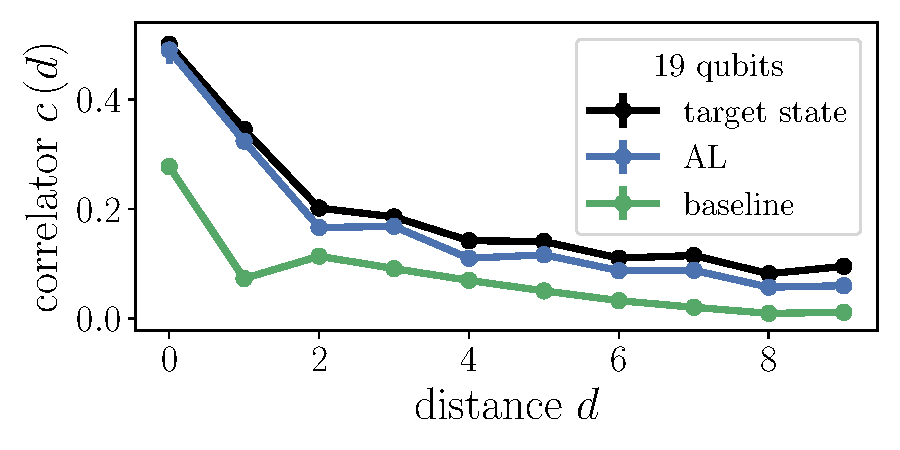
\includegraphics[width=0.45\textwidth]{Paper/Graphics/LGT_different_threshold_correlator_19_qubits.pdf}
   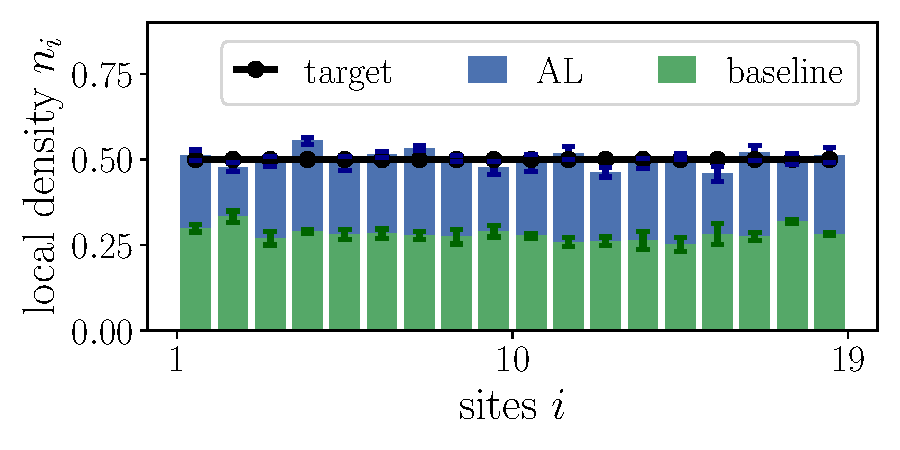
\includegraphics[width=0.45\textwidth]{Paper/Graphics/LGT_different_threshold_density_19_qubits.pdf}
	\caption[]{Correlator over distance (top) and density (bottom) from Eqs. \eqref{eq:GreensSpinDef} and \eqref{eq:LocalDensitySpinDef} for the KCS model state with $h=0$ and $19$ qubits for target state (black) and the reconstructed states using AL (blue) and the baseline (green).}
	\label{fig:LGT_h=0_2}
\end{figure}
% % % % % % % % % % % % % % % % % % % % % % % % % % % 

% % % % % % % % % % % % % % % % % % % % % % % % % % %
\begin{figure}[t]
	\centering
   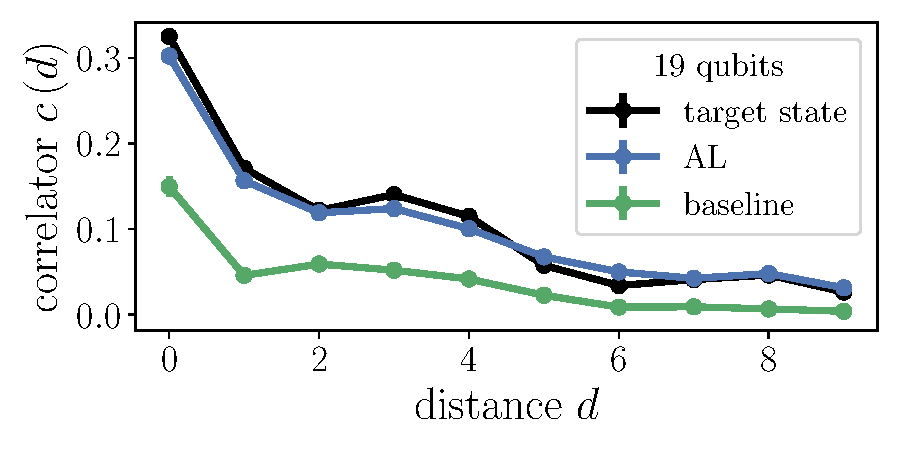
\includegraphics[width=0.45\textwidth]{Paper/Graphics/LGT_h=1_finite_mu_correlator_19_qubits.pdf}
   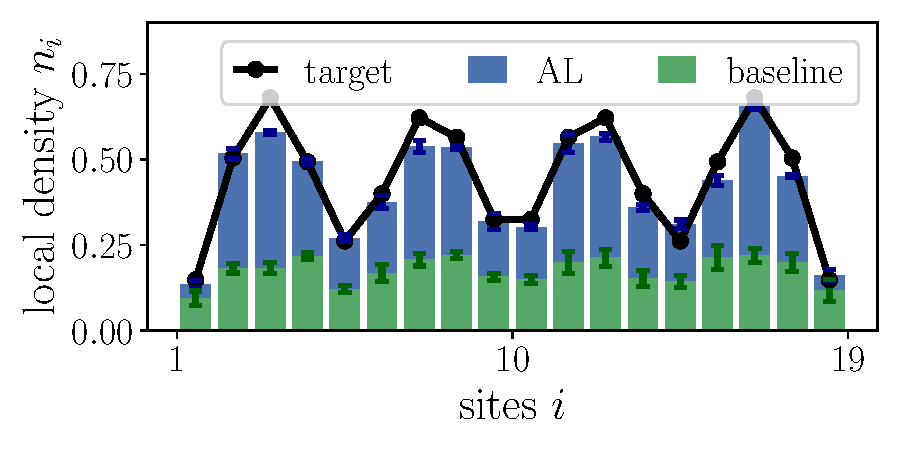
\includegraphics[width=0.45\textwidth]{Paper/Graphics/LGT_h=1_finite_mu_density_19_qubits.pdf}
	\caption[]{Correlator over distance (top) and density (bottom) from Eqs. \eqref{eq:GreensSpinDef} and \eqref{eq:LocalDensitySpinDef} for the KCS model state with $h=1$, $\mu=1$ and $19$ qubits for target state (black) and the reconstructed states using AL (blue) and the baseline (green).}
	\label{fig:LGT_h=1_2}
\end{figure}
% % % % % % % % % % % % % % % % % % % % % % % % % % %


% % % % % % % % % % % % % % % % % % % % % % % % % % %
\begin{figure}[t]
	\centering
\begin{minipage}[t]{0.23\textwidth}
   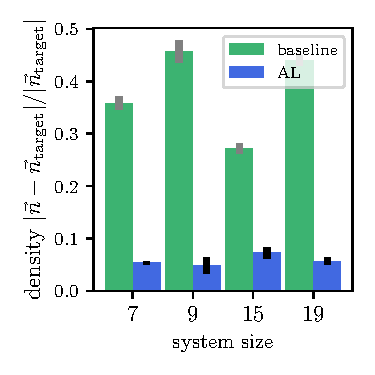
\includegraphics[width=1\textwidth]{Paper/Graphics/LGT_different_threshold_density_difference.pdf}
\end{minipage}
\begin{minipage}[t]{0.23\textwidth}
   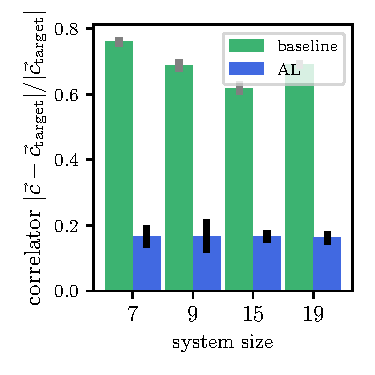
\includegraphics[width=1\textwidth]{Paper/Graphics/LGT_different_threshold_correlator_difference.pdf}
\end{minipage}
	\caption[]{Relative difference of target and reconstructed densities (left) and correlators (right) from Eqs. \eqref{eq:LocalDensitySpinDef} and \eqref{eq:GreensSpinDef} of the KCS model with $h=0$. Error bars correspond to the standard error of the mean.}
	\label{fig:LGT_h=0}
\end{figure}
% % % % % % % % % % % % % % % % % % % % % % % % % % %

% % % % % % % % % % % % % % % % % % % % % % % % % % %
\begin{figure}[t]
	\centering
\begin{minipage}[t]{0.23\textwidth}
   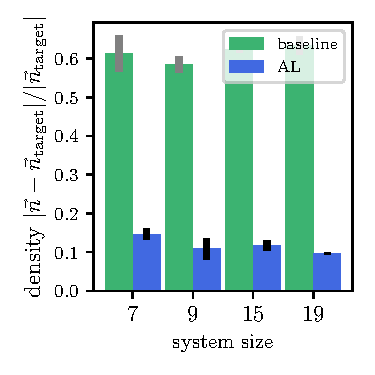
\includegraphics[width=1\textwidth]{Paper/Graphics/LGT_h=1_finite_mu_density_difference.pdf}
\end{minipage}
\begin{minipage}[t]{0.23\textwidth}
   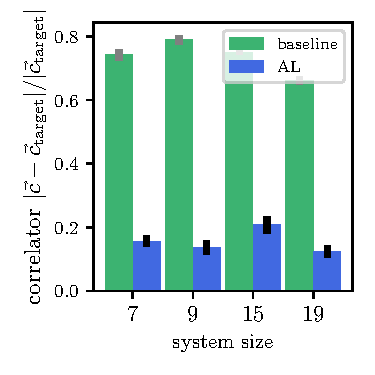
\includegraphics[width=1\textwidth]{Paper/Graphics/LGT_h=1_finite_mu_correlator_difference.pdf}
\end{minipage}
	\caption[]{Relative difference of target and reconstructed densities (left) and correlators (right) from Eqs. \eqref{eq:LocalDensitySpinDef} and \eqref{eq:GreensSpinDef} of the KCS model with $h=1$ and $\mu=1$. An exemplary learning curve for $19$ qubits is shown in the Appendix \ref{appendix:MPS}.}
	\label{fig:LGT_h=1}
\end{figure}
% % % % % % % % % % % % % % % % % % % % % % % % % % %



To investigate the AL reconstruction of many-body quantum states we can use the matrix product state framework for representing quantum states, such as for example the GHZ state and the KCS model states, and sampling in different basis configurations.
In this section, the AL results for these states with $5$ to $19$ qubits are presented in Figs.~\ref{fig:GHZ_pyten} to \ref{fig:LGT_h=1}, with the number of samples and configurations used for the reconstruction from Tab.~\ref{tab:Samples_DMRG}. For all states a commitee of four RBMs and one sample per query were used. 

\subsubsection{Reconstruction of GHZ states}
In Fig.~\ref{fig:GHZ_pyten}, the re-scaled fidelity $1-f^{1/N}$ and the Kullback-Leibler divergence from the same AL learning cycles are shown. The learning was stopped when a re-scaled fidelity of $f^{1/N}_{\mathrm{stop}}$ specified in Tab.~\ref{tab:Samples_DMRG} was reached. For all investigated system sizes the active learner chose $zz\dots z$ as a reference basis. Depending on the system size $50$ to $110$ samples in up to $11$ different measurement configurations were used at the end. In general, the results improve significantly for both quantities when using active learning, i.e. by $30\, \%$ re-scaled fidelity for $5$ qubits or by almost $23\,\%$ for $15$ qubits. Furthermore, the standard deviation of the results indicated by the error bars was highly reduced. 

For the largest system ($15$ qubits) the learning curve is presented in Fig.~\ref{fig:Example_GHZ15_MPS}. Here, the $zyzzzzzxzzzzzzy$ configuration was chosen in the first query. In the second query, more samples from the $zz\dots z$ configuration were requested. We add $10$ ($30$) samples to the pool of samples in the first (second) query and the fidelity is raised from the first learning cycle with $f^{1/N}= 92.42\%$ to $f^{1/N}=93.72\%$. Although this increase of fidelity does not seem very large on the first sight, the results are around $23\%$ above the baseline reconstruction, when choosing the $2$ additional configurations randomly.

\subsubsection{Kinetically constrained spin chain model}

In Figs.~\ref{fig:LGT_h=0_2} to \ref{fig:LGT_h=1} the tomography results for the kinetically constrained spin chain with $t=1$ and $h=0$, $\mu=0$ or respectively $h=1$, $\mu=1$ are summarized. For these states no full state vectors are available and hence the fidelity cannot be used to evaluate the quality of the reconstruction. Instead, we calculate the density and the correlator from Eqs. \eqref{eq:LocalDensitySpinDef} and \eqref{eq:GreensSpinDef} of the reconstructed states as defined in Sec.~\ref{sec:States} and compare them to the values for the target states. We have used the stopping conditions $\frac{\vert \vec{n}-\vec{n}_{\mathrm{target}}\vert}{\vert \vec{n}_{\mathrm{target}}\vert}\leq \tilde{n}_{\mathrm{stop}}=0.2$ and $\frac{\vert \vec{c}-\vec{c}_{\mathrm{target}}\vert}{\vert \vec{c}_{\mathrm{target}}\vert}\leq \tilde{c}_{\mathrm{stop}}=0.2$.


The target and reconstructed density $\vec{n}_{\mathrm{target}}$ and $\vec{n}$ have $N-1$ entries (for each possible domain wall between site $i$ and $i+1$). The spatially resolved domain wall densities for the kinetically constrained spin chain ground states with $h=0$, $\mu=0$ and $h=1$, $\mu=1$ are shown in Figs.~\ref{fig:LGT_h=0_2} and \ref{fig:LGT_h=1_2} (bottom) for a system with $19$ qubits. For $h=0$ and $\mu=0$ the local target density is $n_i=0.5$. For $h=1$ and $\mu=1$, the conserved total system density is equal to $n^{\rm tot} = 8 / 18$ and one can observe Friedel oscillations, where the oscillations are proportional to $k_f = \pi n^{\rm tot}$ \cite{Borla2020}. For both target KCS model ground states the reconstructed states have a domain wall density which agrees with the target density in terms of magnitude and general characteristics (i.e. oscillations) when using AL. In contrast, the baseline without AL results in local densities $n_i$ which are only of around half of the magnitude of the target densities.

A similar tendency can be observed for the target and reconstructed correlators $ \vec{c}_{\mathrm{target}}$ and $\vec{c}$. They have $\lfloor \frac{N}{2}\rfloor$ entries since we calculate the correlator over distance $d$ for the site at the middle of the chain. Also here the baseline reconstruction without AL yields values of $c(d)$ with a much smaller magnitude than for the target state for all distances $d$ and both parameter sets ($h=0$, $\mu=0$ and $h=1$, $\mu=1$). In contrast, when using active learning the reconstructed correlator values are of the same magnitude as for the target state and even follow local features (see bending of the curve in Fig.~\ref{fig:LGT_h=1_2}). Moreover, the power-law for $h=0$ and exponential decay for $h=1$ can be reconstructed when using AL, but not for the baseline (see appendix, Figs.~\ref{fig:LGT_h=0_21} and \ref{fig:LGT_h=1_21}).

To conclude, for the KCS model with $19$ qubits the reconstruction is improved drastically when using AL compared to the baseline scenario. This conclusion can also be drawn from the reconstruction of the KCS model states for other system sizes shown in Figs.~\ref{fig:LGT_h=0} and \ref{fig:LGT_h=1}. 
 For $h=0$ the change of reference basis yields a reduction of the density differences between target and reconstructed state by a factor $5$ for AL, from a relative value of around $44\,\%$ to around $6\,\%$ when averaging over all system sizes. The difference of correlators is decreased from $69\,\%$ to about $17\,\%$.  
For $h=1$ the difference in densities is decreased from an absolute value of around $61\,\%$ to less than $12\,\%$. The difference of target and reconstructed correlators is decreased to around $16\,\%$ from $74\,\%$. For both values of $h$ and all system sizes the active learner selected the $xx\dots x$ configuration as reference basis. This is different from the choice for the usual RBM procedure implemented in QuCumber which always uses the $zz\dots z$ configuration as reference basis. For almost all sizes the stopping condition was reached within the first learning cycle in step 3.)  (except for the $15$ qubit state ($h=0$), where another measurement in the reference basis was requested). Hence, this change of the reference frame by applying active learning already improves the results extremely, even without a need for the further steps 4.) and 5.).\\




% % % % % % % % % % % % % % % % % % % % % % % % % % %
\begin{table}[]
\begin{tabular}{p{1.91 cm}|p{1.3 cm}p{1.3 cm}p{1.3 cm}p{1.3 cm}}
\textbf{GHZ}                & $5$ qubits & $7$ qubits & $9$ qubits & $15$ qubits \\\hline
reference        &    $zz\dots z$      &       $zz\dots z$  &  $zz\dots z$        &    $zz\dots z$      \\
$N_{\mathrm{tot}}$        &    $51$      &       $60$   &  $110$        &    $80$       \\
$N_{\mathrm{queries}}$  & $1$         &    $30$      & $10$         &  $2$  \\  
$N_{\mathrm{per\, query}}$  & $1$         &    $1$      & $1$         &  $10$  \\  
$N_{\mathrm{config}}$  & $2$         &    $4$      & $4$         &  $2$ \\
$f^{1/N}_{\mathrm{stop}}$  & $96\%$         &    $95\%$      & $90\%$         &  $93.5\%$
\end{tabular}
\newline
\vspace*{0.2 cm}
\newline
\begin{tabular}{p{1.91 cm}|p{1.3 cm}p{1.3 cm}p{1.3 cm}p{1.3 cm}}
\textbf{KCS} ($h=0$)                & $7$ qubits & $9$ qubits & $15$ qubits & $19$ qubits \\\hline
reference        &    $xx\dots x$      &       $xx\dots x$  &  $xx\dots x$        &    $xx\dots x$      \\
$N_{\mathrm{tot}}$         &    $200$      &       $200$   &  $202$        &    $500$       \\
$N_{\mathrm{queries}}$  & $0$         &    $0$      & $1$  &  $0$   \\ 
$N_{\mathrm{per\, query}}$  & $-$         &    $-$      & $2$         &  $-$  \\ 
$N_{\mathrm{config}}$  & $1$         &    $1$      & $1$         &  $1$         
\end{tabular}
\newline
\vspace*{0.2 cm}
\newline
\begin{tabular}{p{1.91 cm}|p{1.3 cm}p{1.3 cm}p{1.3 cm}p{1.3 cm}}
\textbf{KCS} ($h=1$)                & $7$ qubits & $9$ qubits & $15$ qubits & $19$ qubits \\\hline
reference   &    $xx\dots x$      &       $xx\dots x$  &  $xx\dots x$        &    $xx\dots x$      \\
$N_{\mathrm{tot}}$         &    $200$      &       $200$   &  $400$        &    $500$       \\
$N_{\mathrm{queries}}$  & $0$         &    $0$      & $0$  &  $0$   \\  
$N_{\mathrm{config}}$  & $1$         &    $1$      & $1$         &  $1$         
\end{tabular}
\caption{Reference configuration selected by the AL, number of samples $N_{\mathrm{tot}}$, number of queries $N_{\mathrm{queries}}$, number of samples per query $N_{\mathrm{per\,query}}$ and configurations $N_{\mathrm{config}}$ selected by the active learner for the reconstruction of the DMRG states: For the kinetically constrained spin (KCS) model ground states, and GHZ states. For the GHZ states, the threshold fidelity for stopping the learning is presented as well. For the KCS states we have used the stopping conditions $ \tilde{n}_{\mathrm{stop}}=0.2$ and $ \tilde{c}_{\mathrm{stop}}=0.2$.}
\label{tab:Samples_DMRG}
\end{table}
% % % % % % % % % % % % % % % % % % % % % % % % % % %








\section{Summary and Outlook \label{sec:Summary}}

In this work, we propose and implement an active learning scheme for adaptive quantum state tomography.
Assuming that the quantum state under consideration has some internal structure, as it is typically the case for states of interest, the active learning scheme uses the information available in the measurement data taken already to propose the basis configuration for the next measurement with the most possible information gain.
We show that for a given number of measurements, our scheme provides a significant improvement in the reconstructed quantum state compared to a random choice of basis configurations. For a quantum state without any structure, the active learning scheme cannot provide an advantage, but will perform as good as a random choice of configurations. 

The active learning scheme is generally applicable to different quantum states and devices, such as trapped ions, neutral atoms in optical tweezers, and superconducting qubits, as shown here. With the increasing number of quantum devices, the need for an efficient way to characterize the realized quantum state arises. Applications range from the verification of quantum computing devices, e.g. testing how faithfully a given quantum state can be prepared, to probing exotic states of matter realized in (analog) quantum simulators, such as the recently realized quantum spin liquid states \cite{Semeghini2021,Satzinger2021}, where measurements in different bases are necessary to characterize the quantum state. 

Apart from the implementation of our protocol in an interactive experimental feedback loop, possible directions for future work include more advanced schemes, e.g. more possible reference bases in the first step. Our active learning scheme can furthermore be generalized to state representations other than the restricted Boltzmann machines considered here, such as variational autoencoders \cite{Rocchetto2018}, recurrent \cite{Morawetz2021} and convolutional neural networks \cite{Schmale2021}, generative adversarial networks \cite{Ahmed2021}, and transformer architectures \cite{Cha2021}.


Another exciting future direction is the combination of the active learning scheme introduced here with the recently proposed classical shadows \cite{Huang2020} by extending the possible active learning actions to different unitary gates, potentially involving two or more qubits.  




%%%%%%%%%%%%%%%%%%%%%%%%%%%%%%%%%%%%%%
\emph{Acknowledgements.--}
We thank Tizian Blatz, Juan Felipe Carrasquilla, Anna Dawid, Ehsan Khatami, Sam Mardazad, Sebastian Paeckel, Henning Schlömer, and Jeffrey Thompson for fruitful discussions. This research was funded by the Deutsche Forschungsgemeinschaft (DFG, German Research Foundation) under Germany's Excellence Strategy -- EXC-2111 -- 390814868, by the European Research Council (ERC) under the European Union’s Horizon 2020 research and innovation programm (Grant Agreement no 948141) — ERC Starting Grant SimUcQuam and by the NSF through a grant for the Institute for Theoretical Atomic, Molecular, and Optical Physics at Harvard University and the Smithsonian Astrophysical Observatory.



%%%%%%%%%%%%%%%%%%%%%%%%%%%%%%%%%%%%%%%%
%% CODE REMOVED BY FABIAN:
    %\bibliography{BibFiles/Lit.bib}
    %\bibliographystyle{unsrt}
    %\bibliographystyle{apsrev4-1}
    %
    %\printbibliography[heading=none]

%% CODE ADDED BY FABIAN:
\bibliography{Lit.bib}
\bibliographystyle{apsrev4-1}

\newpage~
%~\newpage

\appendix 
\section{Quantum state representation in terms of a restricted Boltzmann machine \label{appendix:RBM}}
Part of our active learning scheme is the training of a commitee of restricted Boltzmann machines (see Fig.~\ref{fig:AL}). In this work, the implementation of RBMs within the open-source software python package QuCumber \cite{Qucumber2019} is used for the training. The package is designed to learn quantum many body wave functions from a set of projective measurements in different basis configurations by representing the reconstructed state by RBMs. In this section, we will present how to represent quantum states in terms of RBMs and more details to the RBM training.\\

Firstly, a quantum state $\ket{\Psi}$ with only positive coefficients $\Psi(\vec{x}) = \langle\vec{x} \vert \Psi \rangle \geq 0$ will be considered, where 
$\{\ket{\vec{x}^b}\}$ with $\{\ket{\vec{x}^b}\} = \ket{x_1^b, \dots , x_N^b}$ is a reference basis $b$ for the Hilbert space of $N$ quantum degrees of freedom (i.e. for two qubits it consists of the states $\ket{00}$, $\ket{01}$, $\ket{10}$ and $\ket{11}$). In this case, the representation of a quantum state in terms of a RBM is straight forward: For an infinite number of measurements in a reference basis, i.e. in the $b = z$ basis, the measurements adhere to Born's rule and the probability of finding a measurement result $\vec{x}$ is 
$$
q(\vec{x})=\vert \Psi (\vec{x})\vert^2.$$

QuCumber creates a RBM network with a probability distribution \begin{align}
p_\lambda (\vec{v}) =\frac{1}{Z}\prod_{j=1}^{V}\mathrm{exp}\left( b_j v_j\right) \prod_{i=1}^{H} \left\{ 1 + \mathrm{exp}\left( \sum_j^V W_{ij} v_j +c_i \right)\right\},
\label{eq:RBM_prob2}
\end{align} 
where $\vec{v}$ and $\vec{h}$ are the visible and hidden nodes of the RBM and $W_{ij}$ the weights between visible node $i$ and hidden node $j$ \cite{Goodfellow}. For a finite data set $\mathcal{D}= (\vec{x}_1, \vec{x}_2, \dots)$ it trains the RBM
such that the Kullback-Leibler divergence (see Eq.~\eqref{eq:KL})
is minimized. The minimization is performed by gradient descent, which involves the calculation of expectation values with respect to the distributions of the data and the model. To calculate the expectation value over the model distribution one usually uses Markov Chain Monte Carlo Gibbs sampling. Due to the restricted nature of RBMs hidden and visible units are conditional independent and hence the conditional probabilities factorize. Consequently, it is possible to calculate the conditional distributions of all visible / hidden nodes in parallel by taking $\vec{h}_{t+1} \propto p(\vec{h}\vert \vec{v}_t)$ and $\vec{v}_{t+1} \propto p(\vec{v}\vert \vec{h}_{t+1})$, where $t$ measures the number of steps in the Monte Carlo chain. For large $t\to \infty$ it is guaranteed to converge \cite{Mehta2019}. A slight modification which simplifies the training process is called contrastive divergence. Hereby, only $k$ iterations of Gibbs sampling are performed (contrastive divergence steps).\\


For positive wave functions the RBM representation can be defined as
$$
\psi_\lambda(\vec{x}) = \sqrt{\frac{p_\lambda(\vec{x}}{Z_\lambda}},
$$
with a normalization constant $Z_\lambda$ \cite{Qucumber2019}. 

For more general wave functions with complex-valued coefficients like
\begin{align}
\ket{\Psi} = \sum_{x_1, \dots x_N} \Phi_{x_1, \dots, x_N} \mathrm{e}^{i\varphi_{x_1, \dots, x_N}}\ket{x_1, \dots, x_N}
\label{eq:complex_psi}
\end{align}
the probability distribution underlying the outcomes of projective
measurements in the reference basis does not contain all possible information about the unknown quantum state, because the information about the phase is lost when only considering the underlying probability distribution of measurements in one basis $q(\vec{x})=\vert \Psi (\vec{x})\vert^2$. In this case QuCumber represents the quantum state as defined in Eq.~\eqref{eq:RBMstate}
%\begin{align}
%\psi_{\lambda, \mu}(\vec{x}) = \sqrt{\frac{p_\lambda(\vec{x}}{Z_\lambda}}\mathrm{e}^{i\theta_\mu(\vec{x})/2},
%\end{align}
and trains two RBMs with parameters $\lambda$ and $\mu$ separately. The RBM with parameters $\lambda$ models the amplitude of the RBM wave function, the second RBM with parameters $\mu$ the phase $\theta_\mu(\vec{x}) = \mathrm{log}\, p_\mu(\vec{x})$. Firstly $\lambda$ is optimized such that $\vert \Psi (\vec{x}^b)\vert ^2 = \vert \psi_{\lambda, \mu} (\vec{x}^b)\vert ^2 $ for measurements $\vec{x}^b$ in the reference basis $b$, which is set to the $z$-basis by default. Secondly, measurements in other basis configurations are considered to determine the phase $\theta_\mu$ by training another RBM \cite{Torlai2018}.\\

\begin{figure}[t!]
	\centering
  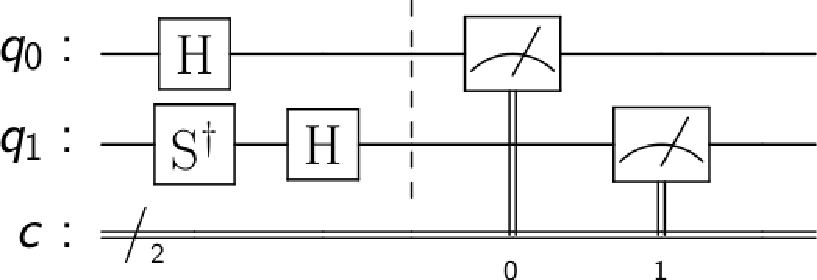
\includegraphics[width=0.4\textwidth]{Paper/Graphics/xy_measurement.pdf}
	\caption[Measurement of a quantum circuit in the $xy$ basis configuration]{Measurement of a quantum system with two qubits ($q_0$ and $q_1$) in the $xy$ basis configuration. Therefore $q_0$ is rotated from the $z$ to the $x$ axis by applying the Hadamard gate, and $q_1$ to the $y$ axis by application of a combination of $S$ and Hadamard gates (see equations \eqref{eq:Hadamard} and \eqref{eq:K}). Figure generated with Qiskit \cite{Qiskit2010}.}
	\label{fig:Configs}
\end{figure}

The information about the phase is extracted via the rotation of single qubits within a quantum circuit into another basis. QuCumber uses by default the $z$ basis as reference basis and rotates to the $x$ and $y$ bases to extract phase information. The rotation of a single qubit to the $x$ basis is achieved by applying the Hadamard gate 
\begin{align}
    H = \frac{1}{\sqrt{2}}\left( \begin{array}{rr}
1 & 1  \\ 
1 & -1 \\
\end{array}\right),
\label{eq:Hadamard}
\end{align}
the rotation to $y$ by applying a combination of the S-adjoint gate and the Hadamard gate,
\begin{align}
    K = \frac{1}{\sqrt{2}}\left( \begin{array}{rr}
1 & -i \\ 
1 & i \\
\end{array}\right).
\label{eq:K}
\end{align}
The rotations are performed by using the pre-defined quantum operations of Qiskit as shown for an exemplary rotation from $zz$ to $xy$ in figure \ref{fig:Configs}.

The representation of a complex wave function in terms of the RBMs as explained above is implemented with the QuCumber package by using the \texttt{ComplexWaveFunction} method.


%%%%%%%%%%%%%%%%%%%%%%%%%%%%%%%%%%%%%%%%%%%%%%%%%%%%%
\section{Details of active learning QST}

%When using the AL procedure as described in section \ref{sec:Model}, one sample per query is used if not stated otherwise ($n_{\mathrm{query}}=1$). If not stated otherwise the active learner did not request the same measurement configuration several times and hence the number of queries $Q=C-1$ is given b the number of configurations $C$ as specified in tables \ref{tab:Samples_DMRG} and \ref{tab:Samples_IBM}. The number of samples at the beginning $n_{\mathrm{start}}$ (step 1.)) can be calculated via the number of samples at the end of the AL, $n_{\mathrm{end}}$ given in the same tables:
%$$n_{\mathrm{start}}=n_{\mathrm{end}}-Q\cdot n_{\mathrm{query}}.$$

When using the AL procedure as described in section \ref{sec:Model}, within each cycle (step 3.)), $4$ RBMs are used if not stated otherwise, with
$1000$ epochs, a learning rate of $l = 0.07$  and contrastive divergence steps $k = 100$.   

\subsection{IBM quantum states \label{appendix:IBM}}

\begin{figure}[htp]
	\centering
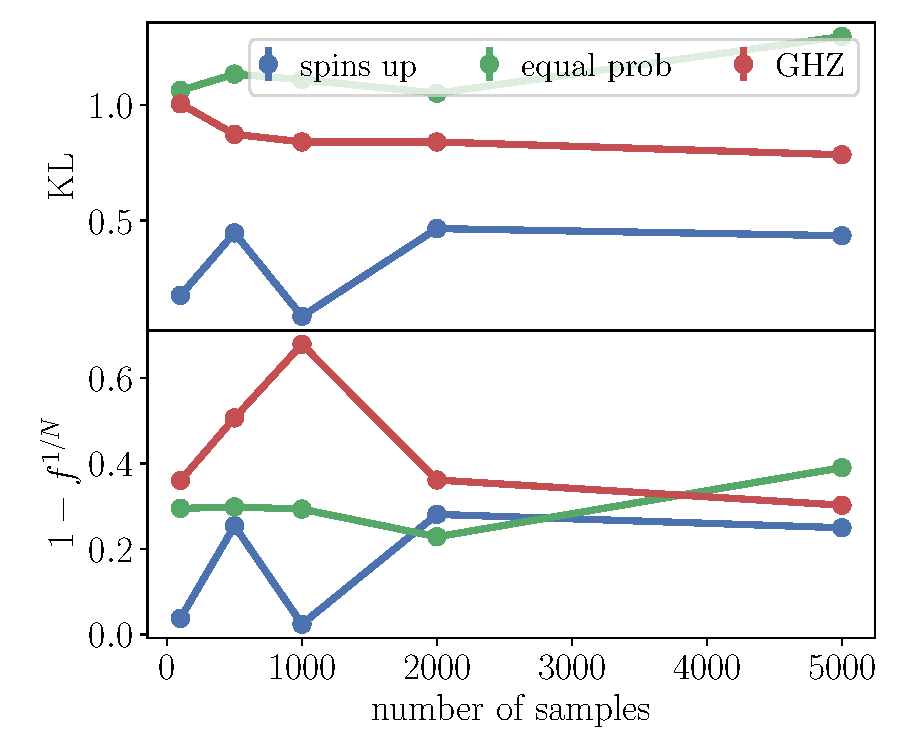
\includegraphics[width=0.5\textwidth]{Paper/Graphics/quantum_test_number_of_samples.pdf}
	\caption[]{Reconstruction results for a pure RBM reconstruction of quantum states prepared on an IBM device ($5$ qubits) without AL. The number of samples is varied by keeping the number of configurations fixed ($6$ configurations).}
\label{fig:WithoutAL1}
\end{figure}
\begin{figure}[htp]
	\centering
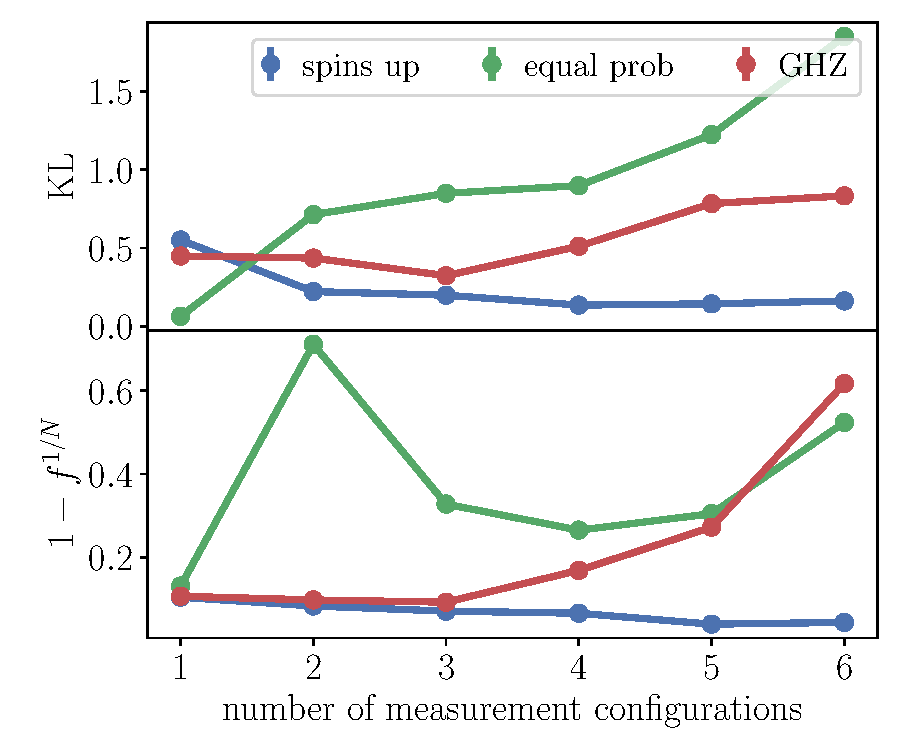
\includegraphics[width=0.5\textwidth]{Paper/Graphics/quantum_test_number_of_configs.pdf}
	\caption[]{Reconstruction results for a pure RBM reconstruction of real quantum states ($5$ qubits) without AL. The number of configurations is varied by keeping the number of samples fixed ($2000$ samples).}
\label{fig:WithoutAL2}
\end{figure}

For the generation of states on a classical quantum simulator we use the Aer simulator, which is designed to  mimic the execution of an actual device \cite{IBM}. For real quantum states the devices \textit{ibmq bogota} and \textit{ibmq quito} were used, which both consist of $5$ superconducting qubits. 

In figures \ref{fig:WithoutAL1} and \ref{fig:WithoutAL2} the results for a pure RBM reconstruction of real quantum states ($5$ qubits) without AL are shown. In \ref{fig:WithoutAL1} the number of samples is varied by keeping the number of configurations fixed ($6$ configurations). In \ref{fig:WithoutAL2} the number of configurations is varied when fixing the number of samples ($2000$ samples). It can be seen that it is difficult and very time consuming to find the most efficient set of measurements and configurations by such scans. Furthermore, the number of samples and configurations with the best reconstruction varies from state to state. This makes our active learning scheme very appreciable since it chooses the number of samples and configurations on its own and only the number of samples at the beginning and per query have to be fixed by the user. As can be seen from section \ref{sec:States} equally good results can be obtained for all states when setting the number of samples per query to $1$ or $2$. Hence, the only free parameter is the number of samples at the beginning of the AL.  
%\begin{figure}[t]
%	\centering
%  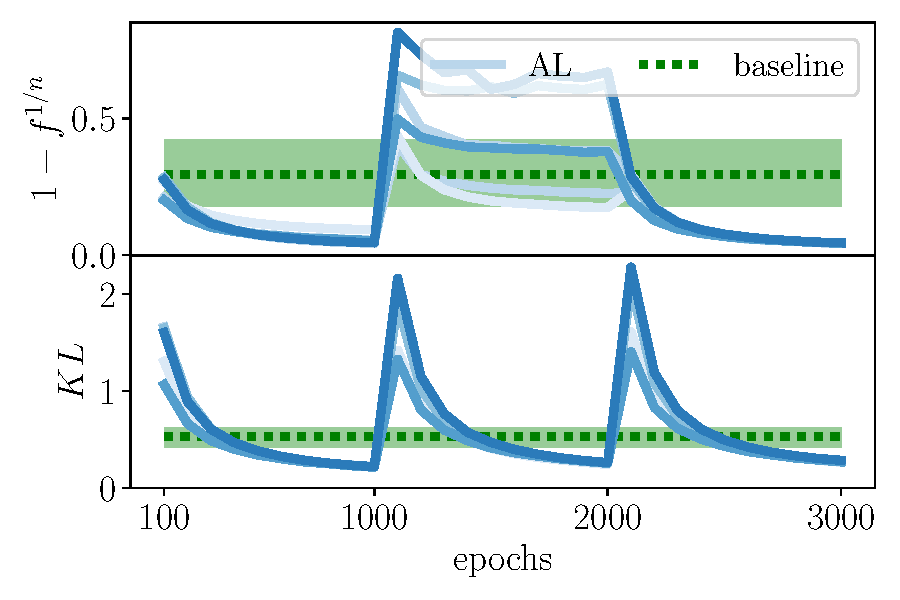
\includegraphics[width=0.48\textwidth]{Paper/Graphics/classical_GHZ.pdf}
%	\caption[]{Examplary learning curves for the GHZ state (see eq. \eqref{eq:State3}) with $5$ qubits generated on a IBM classical quantum simulator.}
%	\label{fig:Example_GHZIBM}
%\end{figure}



%In Fig. ~\ref{fig:Example_GHZIBM} the reconstruction of a GHZ state is shown. One can see that the fidelity is increased from $f^{1/N}_{\mathrm{baseline}}=76\pm 20\,\%$ to $f^{1/N}=91\pm 4\,\%$ when using AL. Furthermore, the span of results for the fidelity is highly reduced. This can be seen by comparison to the first learning cycle of the AL routine (first part in the upper figure of Fig.~\ref{fig:Example_GHZIBM}), but mostly by comparison to the baseline. For the baseline, the results for different results is $40\,\% \leq f^{1/N}_{\mathrm{baseline}} \leq 95\,\%$. In contrast, the deviations are very small for the $KL$, which suggests that for the baseline the RBM training itself works, but the amount of information contained in the training samples from $zzzzz$ and $zyzyy$ configurations (the latter is randomly chosen) is not enough to extract the relevant information for learning the state vector. In contrast, when using AL one measurement from the $yxxxy$ configuration in addition to the $zzzzz$ configuration is requested, which leads to the significant improvement described above.





\subsection{DMRG states \label{appendix:MPS}}



\begin{figure}[t]
	\centering
  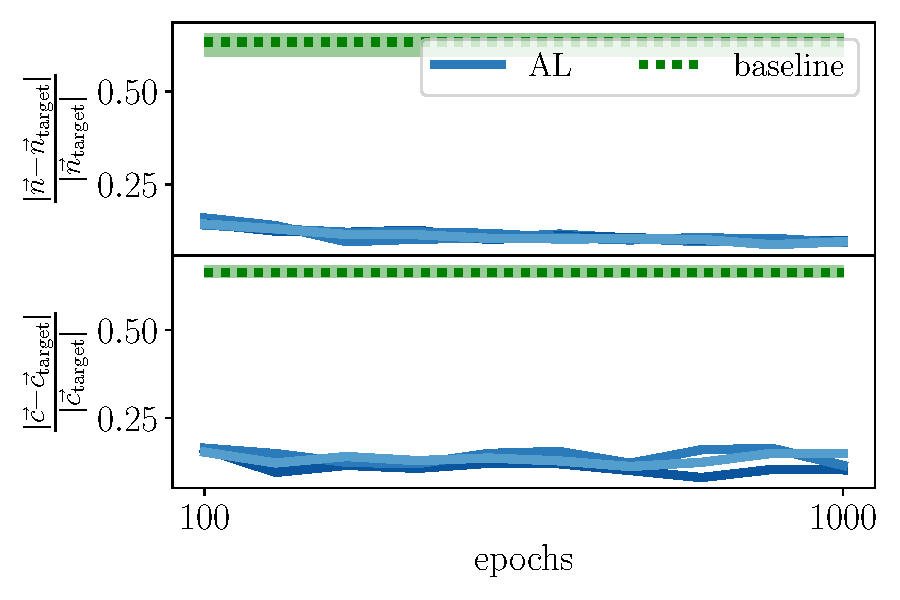
\includegraphics[width=0.48\textwidth]{Paper/Graphics/LGT_h=1_finite_mu_allquantities_19_qubits_summary.pdf}
	\caption[]{Examplary learning curves for a LGT state with $19$ qubits and $h=1$.}
	\label{fig:Example4}
\end{figure}

\begin{figure}[t]
	\centering
   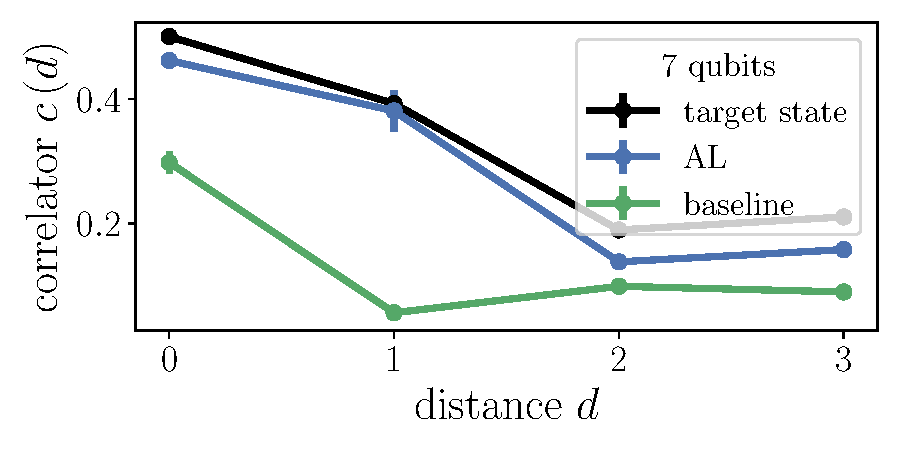
\includegraphics[width=0.45\textwidth]{Paper/Graphics/LGT_different_threshold_correlator_7_qubits.pdf}
   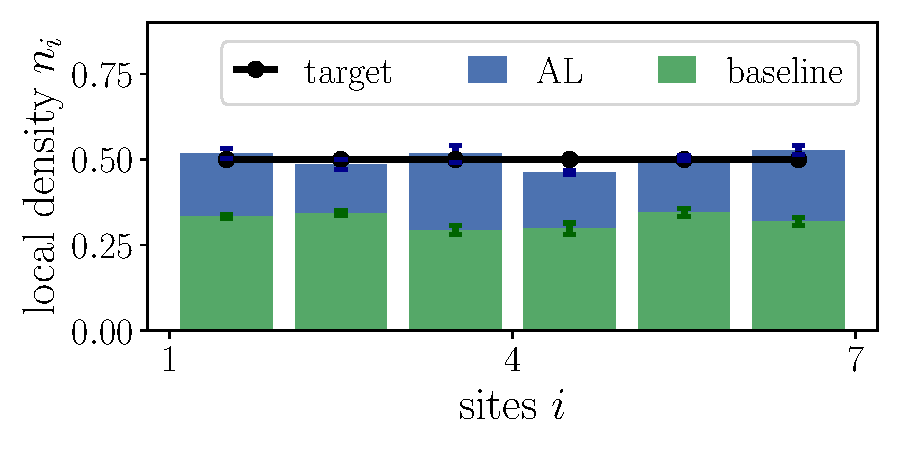
\includegraphics[width=0.45\textwidth]{Paper/Graphics/LGT_different_threshold_density_7_qubits.pdf}
	\caption[]{Correlator over distance (top) and density (bottom) for the KCS state with $h=0$ and $7$ qubits for target state (black) and the reconstructed states using AL (blue) and the baseline (green).}
	\label{fig:LGT_h=0_3}
\end{figure}

\begin{figure}[t]
	\centering
   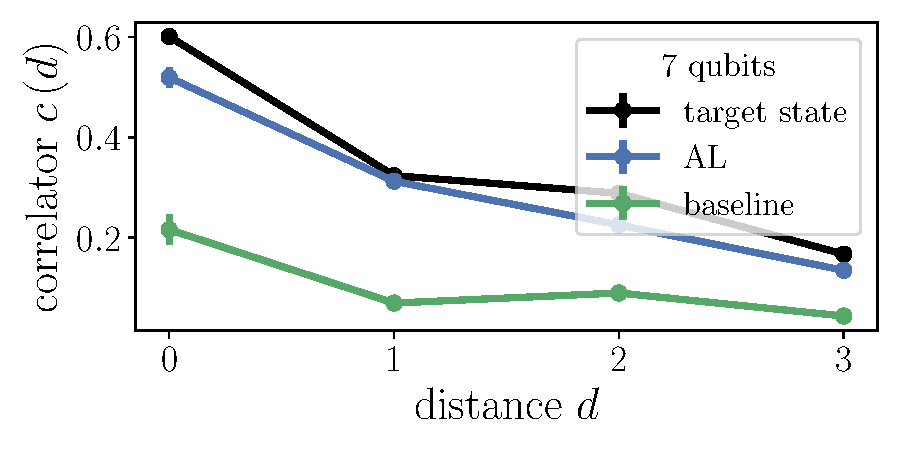
\includegraphics[width=0.45\textwidth]{Paper/Graphics/LGT_h=1_finite_mu_correlator_7_qubits.pdf}
   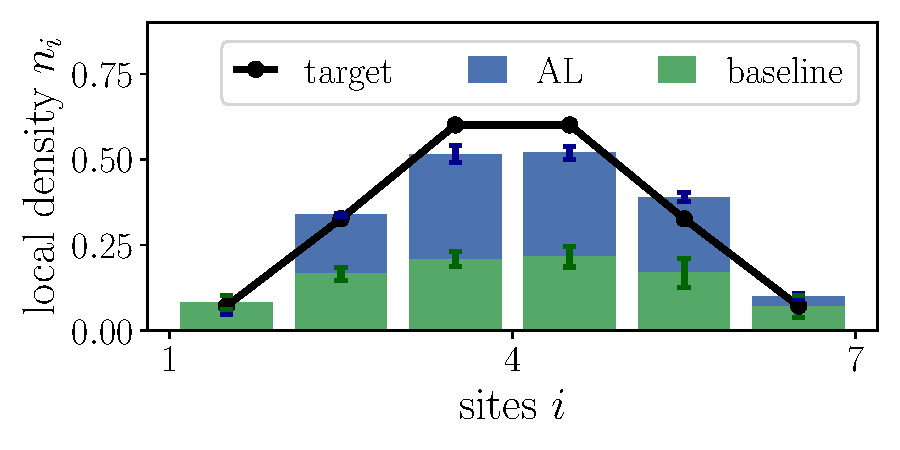
\includegraphics[width=0.45\textwidth]{Paper/Graphics/LGT_h=1_finite_mu_density_7_qubits.pdf}
	\caption[]{Correlator over distance (top) and density (bottom) for the KCS state with $h=1$, $\mu=1$ and $7$ qubits for target state (black) and the reconstructed states using AL (blue) and the baseline (green).}
	\label{fig:LGT_h=1_3}
\end{figure}


For the DMRG states, rotations are performed by applying a rotation matrix 
\begin{align}
    R(\vec{\theta})=e^{i\vec{\theta}\cdot \vec{S}}
\end{align}
to the state. For a rotation of one qubit to the $x$ axis around the $y$ axis this rotation is given by
\begin{align*}
    R_{z\to x}&=R_y\left(\frac{\pi}{2}\right)=\mathrm{exp}\left(i\frac{\pi}{2}S_y\right)=\mathrm{exp}\left(-\frac{\pi}{2}\mathbb{I}\right)\\&=\mathrm{cos}(-\frac{\pi}{2})\mathbb{I}+\mathrm{sin}(-\frac{\pi}{2})\mathbb{I}=-\mathbb{I}= iS_y
\end{align*}
with 
\begin{align*}
    \mathbb{I}=\left(\begin{matrix}
0 & -1 \\
1 & 0 
\end{matrix}\right).
\end{align*}
Similarly one obtains for rotations around $x$ to the $y$ axis
\begin{align*}
    R_{z\to y}= -iS_x.
\end{align*}
These operations are applied locally to each qubit with a truncation error of $10^{-16}$. 

For lattice gauge model states we consider states with $\mu=10^{-7}\approx 0$, since the convergence is much faster than for $\mu=0$. 

In Fig.~\ref{fig:Example4} the learning curve for a lattice gauge model state with $19$ qubits and $h=1$ is shown. When using AL divergence, the $xxxxxxx$ configuration is chosen to be the reference basis. One can see that only this choice of reference basis leads to relatively good results for the density differences (around $15\,\%$, see upper part for epoch $0$) and $17\,\%$ correlator difference (bottom). The RBM training then reduces the density difference further to $\vert \vec{n}-\vec{n}_{\mathrm{target}}/\vert \vec{n}_{\mathrm{target}}\vert= 9.59\pm 0.02\,\%$ and $\vert \vec{c}-\vec{c}_{\mathrm{target}}/\vert \vec{c}_{\mathrm{target}}\vert= 12.4\pm 0.2\,\%$. \\

In Figs.~\ref{fig:LGT_h=0_3} and \ref{fig:LGT_h=1_3} the local correlators over distance $d$ (top) and densities over the system size are shown for KCS states with $7$ qubits and $h=0$, $\mu=0$ and $h=1$, $\mu=1$ respectively. Similarly to the results for $19$ qubits in Figs.~\ref{fig:LGT_h=0_2} and \ref{fig:LGT_h=1_2} one can see that the agreement with the target state is improved when using the AL reconstruction scheme. Also here, features like the curvature of the correlator can be reproduced for AL, but not for the baseline. For the parameters $h=1$ and $\mu=0$ the density increases to a maximum in the middle of the chain. Even though this behaviour can be reproduced by AL and baseline, the results for the baseline are of a around half of the magnitude of the target state. In contrast, the AL reconstruction yields densities with magnitudes much closer to the target state.

Moreover, when plotting the correlators for $h=0$ ($h=1$) with logarithmic scales for $x$ and $y$ axes ($y$ axis) as shown for a system with $19$ qubits in Fig.~\ref{fig:LGT_h=0_21} (Fig.~\ref{fig:LGT_h=1_21}) one can observe the expected power-law (exponential) decay for the target state. This power-law (exponential) decay is reconstructed when using AL, but not for the baseline.




\begin{figure}[t]
	\centering
   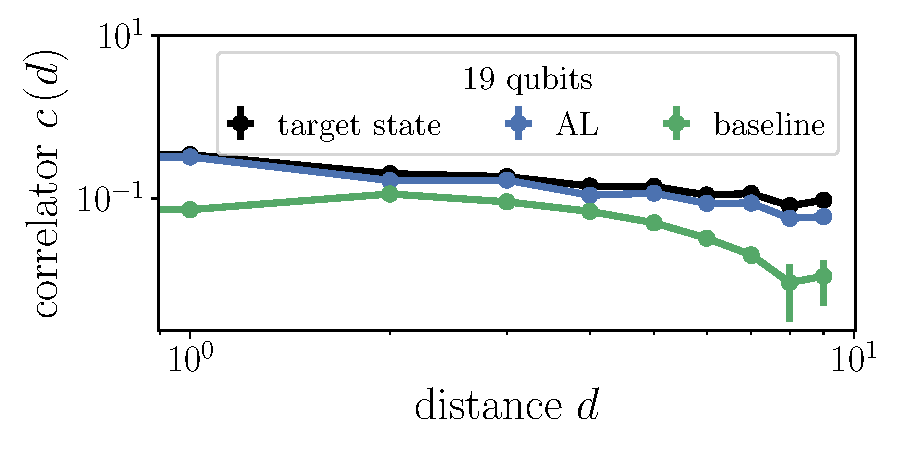
\includegraphics[width=0.45\textwidth]{Paper/Graphics/LGT_different_threshold_correlator_19_qubits_log.pdf}
	\caption[]{Correlator over distance for the KCS model state with $h=0$, $\mu=0$ and $19$ qubits for target state (black) and the reconstructed states using AL (blue) and the baseline (green) as in Fig.~\ref{fig:LGT_h=0_2} but with logarithmic scaling for $x$ and $y$ axes.}
	\label{fig:LGT_h=0_21}
\end{figure}

\begin{figure}[t]
	\centering
   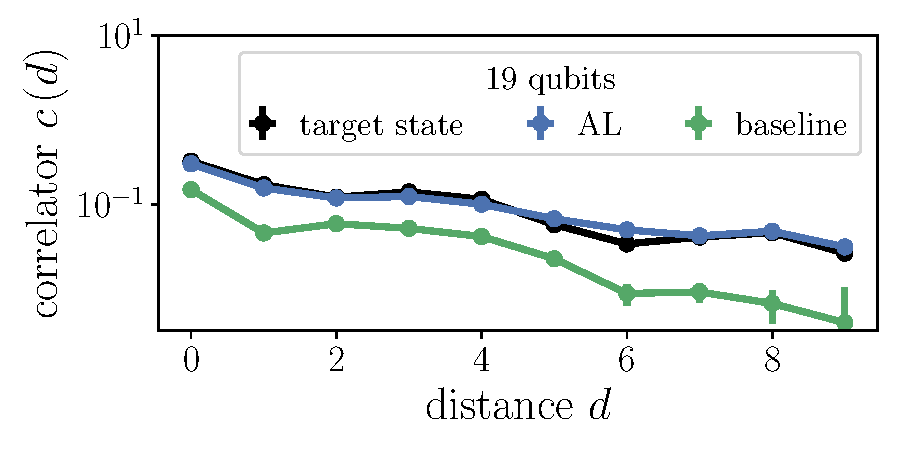
\includegraphics[width=0.45\textwidth]{Paper/Graphics/LGT_h=1_finite_mu_correlator_19_qubits_log.pdf}
	\caption[]{Correlator over distance for the KCS model state with $h=1$, $\mu=1$ and $19$ qubits for target state (black) and the reconstructed states using AL (blue) and the baseline (green) as in Fig.~\ref{fig:LGT_h=1_2} but with logarithmic scaling for the $y$ axis.}
	\label{fig:LGT_h=1_21}
\end{figure}
%%%%%%%%%%%%%%%%%%%%%%%%%%%%%%%%%%%%%%%%%%%%%%%%%%%%%



%%%%%%%%%%%%%%%%%%%%%%%%%%%%%%%%%%%%%%%%%%%%%%%%%%%%%
\section{Kinetically constrained spin model and $\mathbb{Z}_2$ lattice gauge theory}
\label{ApdxKinConsSpn}
%%%%%%%%%%%%%%%%%%%%%%%%%%%%%%%%%%%%%%%%%%%%%%%%%%%%%
In this section we provide more background information on the kinetically constrained quantum spin model, see Eq.~\eqref{eq:LGT_Model_Spin_Def}, considered in the main text.

%%%%%%%%%%%%%%%%%%%%%%%%%%%%%%%%%%
\subsection{Mapping to a $\mathbb{Z}_2$ lattice gauge theory}
The model in Eq.~\eqref{eq:LGT_Model_Spin_Def} can be mapped to a one-dimensional \Zt lattice gauge theory model, with U(1) matter \cite{Borla2020,Kebric2021}. To this end, domain walls in the spin model are mapped to hardcore bosons, which are coupled to \Zt gauge fields defined on the links between the lattice sites $i,j$. As explained below, one obtains the following equivalent Hamiltonian,
\begin{equation}
    \H_{\mathbb{Z}_2} = -t \sum_{\langle i, j \rangle} \l \ad_i \hat{\tau}^{z}_{\langle i, j \rangle} \a_j + \hc \r
    - h \sum_{\langle i, j \rangle}
    \hat{\tau}^{x}_{\langle i, j \rangle}
    + \mu \sum_{\langle i, j \rangle} \hat{n}_j.
    \label{eq:LGT_Model_Original_Def}
\end{equation}
Here $\ad_j$ is the hardcore boson creation operator, defined on site $j$, and $\hat{n}_j = \ad_j \a_j$ is the local number operator. The \Zt gauge and electric fields are represented with the Pauli matrices, defined on the links between neighboring lattice sites, as $\hat{\tau}^{z}_{\langle i, i+1 \rangle}$ and $\hat{\tau}^{x}_{\langle i, i+1 \rangle}$ respectively. This model is appealing since it exhibits confinement of dynamical particles which is induced by any nonzero \Zt electrical field term $h \neq 0$ \cite{Borla2020,Kebric2021}.

The generator of the local \Zt gauge symmetry of Eq.~\eqref{eq:LGT_Model_Original_Def} can be written as \cite{Prosko2017}
\begin{equation}
    \hat{\mathcal{G}}_j = \hat{\tau}^{x}_{\langle i-1, i \rangle}
    (-1)^{\hat{n}_i} \hat{\tau}^{x}_{\langle i, i+1 \rangle}, \qquad [\H_{\mathbb{Z}_2},\hat{\mathcal{G}}_j]=0.
    \label{eq:GaussLaw}
\end{equation}
This leads to the \Zt Gauss law, requiring all states to be $+1$ eigenstates of $\hat{\mathcal{G}}_j$ (we assume no background charges):
\begin{equation}
    \hat{\mathcal{G}}_j \ket{\psi} = + \ket{\psi}.
    \label{eq:GaussLawConstr1}
\end{equation}

From here it is relatively straightforward to obtain back the constrained spin model Eq.~\eqref{eq:LGT_Model_Spin_Def} from the main text. One notices that the charge configuration is entirely determined by the \Zt electric fields due to the constraints imposed by the \Zt Gauss law. This allows to formulate the Hamiltonian entirely in terms of the gauge field, by identifying  the presence of a particle on a lattice site as anti-alignment of the \Zt electric field defined on the links connecting that site. This also means that the particles, or domain walls, are connected with the \Zt electric fields of the same orientation, which we interpret as strings and anti-strings which connect the \Zt charges.

Using the above interpretation it is straightforward to see that the first term in model \eqref{eq:LGT_Model_Spin_Def} corresponds to the kinetic term, where the number of domain walls is conserved. This ensures two things in the lattice gauge interpretation: the \Zt electric string remains attached to the hopping particle, and the total number of particles is conserved.
The second term $\propto h$ in Eq.~\eqref{eq:LGT_Model_Spin_Def} induces energy cost to strings and as a result confines the particle pairs into dimers. Finally, the Ising term is needed to control the number of domain walls and thus the filling of the chain in the 1D LGT interpretation. 

%%%%%%%%%%%%%%%%%%%%%%%%%%%%%%%%%%
\subsection{The gauge-invariant equal-time Green's function}

The correlation function in Eq.~\eqref{eq:GreensSpinDef} can be mapped to the \Zt invariant equal-time Green's function defined as
\begin{equation}
    {\vec{c}(|i-j|) = \left \langle \ad_i \prod_{i \leq l < j} \hat{\tau}^{z}_{\langle l, l+1 \rangle} \a_j \right \rangle}.
\end{equation}
This is once again done by taking into account the constraint imposed by the Gauss law in Eq.~\eqref{eq:GaussLawConstr1}.
Both terms  $\propto \l 1 \pm 4\hat{S}^{x}_{l}\hat{S}^{x}_{l+1}\r, l \in \{i, j \}$ act as projectors to the states where there is a site with a particle to be annihilated and an empty site, where a particle can be created. The actual annihilation at site $j$ and creation of the particle at site $i$ comes from the application of $\prod_l \l 2 \hat{S}^{z}_l \r$ between the domain walls. Combining both terms, first applying the projectors and then performing the annihilation and creation of the particle, gives us the \Zt Green's function expressed entirely in terms of gauge fields.
Note that the order is slightly changed in the main text Eq.\eqref{eq:GreensSpinDef} by considering the spin anticommutation property.


Such correlation function probes the confinement of particle pairs in the LGT interpretation. It decays as a power law in the deconfined phase $h = 0$ and decays exponentially in the confined phase, which is the case for any non-zero value of the field \cite{Borla2020, Kebric2021}. On the other hand, the pair-pair correlation function decays as a power-law function also in the confined phase, which means that the effective dimers behave as Luttinger liquid \cite{Borla2020}.




\end{document}